
\maketitle

\section{Introduction}
Multiscale phenomena are ubiquitous across natural and engineered systems, arising in fluid dynamics, neuroscience, material science, and biological transport~\cite{jost2005dynamical,wiggins2003introduction}. These systems typically involve a vast number of degrees of freedom, making direct analysis and simulation at the microscopic level prohibitively expensive. Statistical mechanics provides a powerful framework for addressing this complexity by shifting attention from individual particles or agents to their emergent collective behavior~\cite{hill2013statistical}. Within this framework, mean-field theory, introduced by Kac~\cite{kac1956foundations,mckean1966class}, has become a particularly influential tool, offering a principled bridge between microscopic interactions and macroscopic evolution. The mean-field limit replaces the high-dimensional coupled dynamics of $N$ interacting agents with a single representative equation whose drift depends on the law of the process itself, a formulation known as the McKean--Vlasov stochastic differential equation. On the theoretical side, substantial progress has been made on well-posedness~\cite{de2020strong,huang2019distribution}, existence and uniqueness of solutions~\cite{mishura2020existence}, and propagation of chaos~\cite{sznitman2006topics,chaintron2021propagation,jabin2017mean}. On the applied side, mean-field models have found successful applications in areas ranging from mean-field control~\cite{buckdahn2017mean} and mean-field games~\cite{ding2022mean} to high-dimensional sampling~\cite{liu2017stein,carrillo2024fisher} and neural network training~\cite{rotskoff2022trainability}.

Despite this broad success, mean-field modeling faces substantial challenges in practice. Complex systems operating in strongly nonlinear, heterogeneous, or transitional regimes are difficult to describe accurately using simplified effective dynamics alone~\cite{sznitman2006topics,jabin2018quantitative,cattiaux2008probabilistic}. Even when the dominant mechanisms are reasonably well understood, model error, uncertainty in initialization, and unresolved interactions can accumulate over time, leading to significant forecast drift. A natural strategy to mitigate this issue is data assimilation, which continuously incorporates observational information into the model evolution to correct deviations from the true dynamics.

Data assimilation has a long and rich history, particularly in numerical weather prediction and geophysical forecasting. The two dominant paradigms are sequential filtering and variational methods. The Ensemble Kalman Filter (EnKF)~\cite{evensen2003ensemble,evensen2009data} and its many variants approximate the Bayesian filtering distribution by propagating an ensemble of model states and updating them using a Kalman-type correction. Variational methods such as 3D-Var and 4D-Var~\cite{lorenc1986analysis,courtier1994strategy} seek the trajectory that minimizes a cost functional balancing background information and observational fit over a time window. Particle filters~\cite{de2004sparse,chopin2020introduction} provide a fully nonlinear alternative but suffer from weight degeneracy in high dimensions. More recently, feedback-based approaches---commonly referred to as nudging or synchronization methods~\cite{azouani2014continuous,bessaih2015continuous}---have attracted renewed attention due to their simplicity and amenability to rigorous analysis. In nudging, a relaxation term continuously drives the model state toward consistency with observations, and convergence can often be established under verifiable spectral-gap or dissipativity conditions~\cite{albanez2016continuous,jolly2017data}. 

Applying data assimilation to many-body or mean-field systems introduces a fundamental difficulty that is largely absent in classical settings: the model and the observations typically live on different scales. The underlying dynamics are formulated microscopically---in terms of particles or agents such as atoms, molecules, cells, or individual animals---whereas the available data usually consist of macroscopic quantities such as density, momentum, or velocity fields. For example, This scale mismatch renders standard assimilation strategies difficult to apply directly. Updating particle-level states using macroscopic data is not only computationally expensive but also statistically unstable in high-dimensional settings. Classical methods such as EnKF and 4D-Var are generally designed for finite-dimensional state representations with observation operators acting on the same scale as the forecast model, and mean-field systems violate both assumptions.

Several recent efforts have begun to address data assimilation in the context of interacting particles and McKean--Vlasov dynamics, though typically under different settings from the cross-scale scenario considered here. The ensemble Kalman--Bucy filter has been studied in the mean-field limit~\cite{de2018long,del2017stability}, establishing connections between the EnKF update and McKean--Vlasov dynamics; however, these analyses focus on the self-consistency of the filter rather than on assimilating macroscopic observations into microscopic models. Feedback particle filters~\cite{yang2011mean} construct control-theoretic updates for nonlinear filtering, but their extension to the mean-field regime with coarse-grained observations remains largely open. In the PDE-constrained setting, data assimilation for the Navier--Stokes and related dissipative equations via continuous nudging has been extensively studied~\cite{azouani2014continuous,albanez2016continuous,jolly2017data,bessaih2015continuous}, and our framework can be viewed as extending this philosophy to the McKean--Vlasov setting where the state is a probability measure rather than a deterministic field. To the best of our knowledge, a rigorous and computationally scalable framework for cross-scale data assimilation---where macroscopic observations are systematically fed back into microscopic mean-field dynamics---has not been previously established. The present work aims to fill this gap.

A central ingredient of our construction is the Wasserstein gradient-flow interpretation of the nudging term. The theory of gradient flows in the space of probability measures equipped with the Wasserstein metric, pioneered by Jordan, Kinderlehrer, and Otto~\cite{jordan1998variational} and developed extensively by Ambrosio, Gigli, and Savar\'{e}~\cite{ambrosio2005gradient}, provides a variational framework for a broad class of evolution equations including the Fokker--Planck equation, porous medium equations, and aggregation-diffusion models~\cite{carrillo2003kinetic,carrillo2019aggregation}. In this formulation, the evolution of a probability measure is driven by the steepest descent of a free energy functional with respect to the Wasserstein-2 distance.  In our setting, we define the nudging term as the Wasserstein gradient of a quadratic observation-misfit functional, which naturally produces a velocity field that transports the forecast distribution toward the observed one while preserving the conservative structure of the underlying mean-field dynamics.

In this work, we introduce a cross-scale data assimilation framework, termed \emph{Multiscale Nudge}, that addresses the gap between microscopic mean-field dynamics and macroscopic observations. The main contributions are as follows.
\begin{enumerate}
    \item \textbf{Framework.} We propose a nudging mechanism derived from the Wasserstein gradient flow of a regularized observation-misfit functional. The regularization, realized through a smoothing kernel that matches the observation scale, ensures that the feedback acts at the appropriate resolution while preserving the mean-field structure. The resulting assimilated dynamics admit both a measure-valued (Fokker--Planck) and a particle-level (SDE) formulation, and accommodate two practically important observation modalities: pixel-level density reconstructions and unlabeled partial particle locations.
    \item \textbf{Well-posedness and mean-field convergence.} We establish well-posedness of the assimilated McKean--Vlasov SDE under Lipschitz conditions on the model drift and the smoothing kernel. We further prove propagation of chaos for the interacting particle approximation, providing quantitative $N$-dependent error bounds via a synchronous coupling argument.
    \item \textbf{Error estimates.}  We show that the $L^2$ error between the assimilated and true densities decays exponentially to a neighborhood determined by the model bias, provided the nudging intensity is sufficiently large relative to the advection instability.
    \item \textbf{Numerical validation.} We demonstrate the effectiveness of the framework on problems of increasing complexity: a linear Gaussian benchmark with analytical solutions, a bistable bimodal system exhibiting spontaneous symmetry breaking, the Vlasov--Poisson system (Landau damping and two-stream instability), and a real collective-motion dataset of approximately 1000 fish~\cite{walter2021trex}. In each case, the nudging term successfully corrects the biased forecast using only macroscopic density observations.
\end{enumerate}


\section{Method}
Let $(\Omega, \mathcal{F}, \mathbb{P})$ be a probability space with a filtration $(\mathcal{F}_t)_{t \ge 0}$. We consider the reference (ground-true) dynamics governed by the following McKean-Vlasov stochastic differential equation 
\begin{equation}\label{equ:true_mean_field}
\intd \bX_t  = \bb_{\mathrm{true}} (\bX_t,\mu_t)\intd t + \Sigma\intd \bW_t \quad \bX_0 \sim \mu_0
\end{equation}
where $\mu_t= \mathrm{Law}(\bX_t)\in \mathcal P_2(\mathbb R^d)$ denotes the probability distribution of the true process, $\bX_t\in \mathbb R^d$ is the state of the reference particle, $\bW_t$ is a standard $d$-dimensional Brownian motion, $\bb_{\mathrm{true}}:\mathbb R^d\times \mathcal P_2(\mathbb R^d)\to \mathbb R^d$ is the true drift term and $\Sigma  \in \mathbb R^{d\times d}$ is the diffusion coefficient (assumed constant for simplicity). The evolution of $\mu_t$ is given by 
\begin{equation}\label{equ:true_density}
\partial_t \mu_t
= -\nabla_{\mathbf{x}} \cdot \big( \mathbf{b}_{\mathrm{true}}(\mathbf{x},\mu_t),\mu_t \big)+\frac{1}{2}\nabla_{\mathbf{x}} \cdot \big( \Sigma \Sigma^\top \nabla_{\mathbf{x}} \mu_t \big).
\end{equation}
Equation \eqref{equ:true_mean_field} can be viewed as the mean-field approximation of an interacting particle system 
\[
\intd \bX_t^i  = \bb(\bX_t^1,\cdots, \bX_t^N)\intd t  + \Sigma \intd \bW_t^i,
\]
with $N\to \infty$, under appropriate assumptions ensuring propagation of chaos. In practice, the true drift $\bb_{\mathrm{true}}$ is typically unknown. Instead, one has access to an approximate model drift $\bb_{\mathrm{model}}$, which introduces a model error:
\[
\bR(\bx,\mu) := \bb_{\mathrm{model}}(\bx,\mu) -  \bb_{\mathrm{true}}(\bx,\mu).
\]
The corresponding approximate dynamics are given by
\[
\intd \bY_t = \bb_{\mathrm{model}}(\bY_t,\mu^{\mathrm{model}}_t)\intd t + \Sigma \intd \bW_t,
\]
where $\mu^{\mathrm{model}}_t = \mathrm{Law}(\bY_t)$ or, at the particle level,
\begin{equation}
\intd \bY^{i,N}_t = \bb_{\mathrm{model}}(\bY^{i,N}_t,\mu^{\mathrm{model},N}_t)\intd t + \Sigma \intd \bW^{i,N}_t,
\end{equation}
where $\mu^{\mathrm{model},N} = \frac{1}{N}\sum_{i=1}^N \delta_{\bY_i}$. 
Due to errors in initialization and inherent model bias, the discrepancy between the true and approximate systems tends to accumulate over time. Data assimilation offers a natural strategy to mitigate this drift by continuously incorporating observational information into the model evolution. 

However, in the mean-field setting, a fundamental difficulty arises: the representative particle $\bX_t$ is not itself a physical observable, and even in the interacting particle system $\{\bX_t^i\}_{i=1}^N$, individual trajectories are rarely accessible. In many practical applications, the available measurements take the form of aggregate or image-based data—such as density fields reconstructed from pixel observations—from which one cannot establish a correspondence between observed positions and particle indices. For example, in collective motion experiments such as \cite{ballerini2008interaction, cavagna2010scale, zhang2010collective}, the accessible quantity is a coarse-grained spatial density reconstructed from imaging data, rather than the full microscopic state of each individual. In geophysical forecasting \cite{evensen2003ensemble}, satellite observations similarly provide smoothed integrals of the atmospheric state distribution. In all these settings, the observational quantity takes the form of a smoothed density. For simplicity, we consider a particular form of smoothed observation
in this paper. Let $K_h (\bx) = h^{-d}K(\bx/h)$ be a smoothing kernel with bandwidth $h>0$, where $K:\mathbb R^d \to \mathbb R_+$. Concretely, we consider two cases. In the first case, one has access to pixel-level image data, from which the observed density is directly reconstructed as
\[
\mu_t^{\mathrm{obs}}(\bz) = \mathcal{O}_h(\mu_t)(\bz) = \int K_h(\bz - \bx)\,\mu_t(\mathrm{d}\bx).
\]
In the second case, only a partial and unlabeled set of particle locations $\{\bX_t^{\mathrm{obs},k,M}\}_{k=1}^M$ is available, without consistent index correspondence across time, and the observed density is approximated by the kernel density estimator
\[
\mu_t^{\mathrm{obs}}(\bz) = \frac{1}{M}\sum_{k=1}^{M} K_h(\bz - \bX_t^{\mathrm{obs},k,M}).
\]
Both cases fit within the same assimilation framework, as the nudging term depends on $\mu_t^{\mathrm{obs}}$ only through its action as a measure.
To reduce the discrepancy induced by initialization and model error,
the data assimilation method \cite{bessaih2015continuous} was proposed to augment the approximate dynamics with a nudging term that drives $\nu_t$ toward consistency with the observations. Specifically, we consider the assimilated dynamics
\begin{equation}\label{equ:assimilated}
\intd\bZ_t
= \bb_{\mathrm{model}}(\bZ_t,\nu_t)\,\intd t
+ \bu_{\mathrm{nud}}(\bZ_t,\nu_t,\mu^{\mathrm{obs}}_t)\,\intd t
+ \Sigma \intd \bW_t
\end{equation}
A natural and structurally consistent choice is to define the nudging term as the Wasserstein gradient flow associated with a quadratic observation-misfit functional
\[
J_{\mathrm{nud}}(\nu,\mu^{\mathrm{obs}}) = \frac{1}{2}\int_{\mathbb{R}^d} \left| \nu(\bz) - \mu^{\mathrm{obs}}(\bz) \right|^2 \intd \bz,
\]
with 
\[
\bu_{\mathrm{nud}}(\bz,\nu_t,\mu^{\mathrm{obs}}_t) =  -\lambda \nabla_{\bz} \left( \frac{\delta J_{\mathrm{nud}}}{\delta \nu}(\bz) \right) = -\lambda \nabla_\bz (\nu-\mu^\mathrm{obs}),
\]
where $\lambda>0$ is the nudging intensity.
If we assume that $\bb_{\mathrm{model}}$ and $\Sigma$ take a special form $$ \bb_{\mathrm{model}}(\bz,\nu) =  -\nabla \left( \frac{\delta F_{\mathrm{model}}}{\delta \nu}\right)(\bz), \quad \Sigma = \sqrt{2\beta} \mathbf{I}, $$ for some functional $F(\mu)$, then we have the assimilated dynamics \eqref{equ:assimilated} can be interpreted as a Wasserstein gradient flow of the free energy 
\begin{equation}\label{equ:free_energy}
\mathcal F_t (\nu) = F_{\mathrm{model}}(\nu) + \lambda J_{\mathrm{nud}}(\nu,\mu_t^{\mathrm{obs}}) + \beta \mathrm{Ent} (\nu),
\end{equation}
where $\mathrm{Ent} (\nu) = \int \nu\log(\nu)\intd \bz$.
Although the assimilated dynamics \eqref{equ:assimilated} is natural, its theoretical analysis is challenging, since $\nu_t$
is, in general, only a probability measure, whereas well-posedness typically requires regularity and growth assumptions on both $\bb_{\mathrm{model}}$ and $\bu_{\mathrm{und}}$. Motivated by this regularity gap, we introduce a regularization of the free energy~\eqref{equ:free_energy} that nudges the system only at the
observation scale. Specifically, we define
\[
J_{\mathrm{nud},h}(\nu,\mu^{\mathrm{obs}}) = \frac{1}{2}\int_{\mathbb{R}^d} \left| (K_h*\nu)(\bx) - \mu^{\mathrm{obs}}(\bx) \right|^2 \intd \bx,
\]
Computing the F\`echet derivative of $J_{\mathrm{nud},h}$ with respect to the measure $\nu$, denoted as $\frac{\delta J_{\mathrm{nud},h}}{\delta \nu}$, yields:
\[\frac{\delta J_{\mathrm{nud},h}}{\delta \nu}(\bx) = \left( \tilde K_h * \nu - K_h* \mu^{\mathrm{obs}} \right)(\bx),
\]
where $\tilde{K}_h = K_h * K_h$. Note that $\tilde{K}_h$ is
automatically symmetric whenever $K$ is symmetric.
The corresponding nudging velocity is therefore
\[
\bu_{\mathrm{nud},h}(\bz, \nu, \mu^{\mathrm{obs}})
= -\lambda\,\nabla_{\bz} \frac{\delta J_{\mathrm{nud},h}}{\delta \nu}(\bz)
= -\lambda\,\nabla \bigl( \tilde K_h * \nu
  - K_h * \mu^{\mathrm{obs}} \bigr)(\bz).
\]
Substituting into~\eqref{equ:assimilated}, we obtain the regularized assimilated dynamics
\begin{equation}\label{equ:assimilated_regularized}
\intd\bZ_t
= \bb_{\mathrm{model}}(\bZ_t,\nu_t)\,\intd t -\lambda  \nabla \left( \tilde K_h * \nu - K_h * \mu^{\mathrm{obs}} \right)(\bz)\,\intd t
+ \Sigma \intd \bW_t.
\end{equation}
Formally, the Law of $\bZ_t$, denoted by $\nu_t$, satisfies the following nonlinear Fokker-Planck equation:
\begin{equation}\label{equ:fpk_regularized}
\partial \nu _t = -\nabla\cdot \left(\nu_t\bbm(\bx,\nu_t)\right) + \nabla \cdot \left(A \nabla \nu_t \right)+\lambda \nabla \cdot \left( \nu_t \nabla \left( K_h * r \right) \right),
\end{equation}
where $A = \Sigma\Sigma^\top$ and $r = K_h * \nu_t - \mu^{\mathrm{obs}}_t$.
Let us take $K$ as the Gaussian kernel, then we have the following lemma.
\begin{lemma}\label{lemma:kernel}
    For every $h>0$, and a periodical domain $\Omega=\mathbb T^d$, if we choose \(K(\bx) =\pi^{-\frac{d}{2}} \exp(-\|\bx\|^2)\), then for  \[
    K_h(\bx) = h^{-d}K(\bx/h), \quad \tilde K_h = K_h * K_h,
    \]  we have that 
    \begin{enumerate}
        \item $\tilde K_h \in C^{\infty}(\Omega)$ and $\tilde K_h$ is global Lipschitz.
        \item $\nabla \tilde K_h\in L^\infty(\Omega)$ 
        \item For any $v\in H^1(\Omega)$, we have that 
        \[
        \|\nabla v - \nabla (\tilde K_h *v)\|_{L^2(\Omega)} \to 0.
        \] Moreover, if $v\in H^2(\Omega)$, then there exist a constant $C>0$, independent of $h$, such that 
        \[
        \|\nabla v-\nabla(\tilde K_h*v)\|_{L^2(\Omega)}
\le Ch\|D^2 v\|_{L^2(\Omega)}.
        \]
    \end{enumerate}
\end{lemma}
The proof is standard and will be included in the Appendix for the sake of completeness.
Based on the properties of the kernel, we have the following well-posedness result.
\begin{assumption}\label{ass:regularity}
Let us assume the $\bb_{\mathrm{model}}$ and $\bb_{\mathrm{true}}$ satisfies

\medskip
\noindent\textbf{(A1) Bounded model drift.}
There exists a constant $B_{\mathrm{model}}>0$ such that for all $\rho\in\mathcal P_2(\Omega)$,
\[
\|\bbm(\cdot,\rho)\|_{L^\infty(\Omega)} \le B_{\mathrm{model}},
\qquad
\|\nabla\cdot \bbm(\cdot,\rho)\|_{L^\infty(\Omega)} \le B_{\mathrm{model}} .
\]

\medskip
\noindent\textbf{(A2) Lipschitz drift.}
Let us assume that $\bb_{\model}$ is globally Lipschitz:
There exists a constant $L_\model>0$ such that for all $x,y\in\Omega$ and all $\rho,\rho'\in\mathcal P_2(\Omega)$,
\[
\|\bbt(x,\rho)-\bbt(y,\rho')\| \le L_{\true}(\|\bx_1-\bx_2\|+W_2(\rho_1,\rho_2)) .
\]
and
\[
\|\bbm(x,\rho)-\bbm(y,\rho')\| \le L_{\model}(\|\bx_1-\bx_2\|+W_2(\rho_1,\rho_2)) .
\]
% \medskip
% \noindent\textbf{(A3) Bounded densities and positivity.}
% The true density is uniformly bounded, and the assimilated density is uniformly bounded below: there exist constants $\bar\rho>0$ and $\underline\nu>0$ such that, for all $t\ge 0$,
% \[
% \|\mu_t\|_{L^\infty(\Omega)} \le \bar\rho,
% \qquad
% \nu_t(x)\ge \underline\nu \ \text{for a.e. }x\in\Omega .
% \]

\end{assumption}

\begin{proposition}[Well-Posedness of Equation \eqref{equ:assimilated_regularized}]\label{prop:well_possedness}
Let us assume that $\bb_{\model}$  is globally Lipschitz: there exist $c>0$, such that for any $\bx_1,\bx_2 \in \mathbb R^d $ and $\nu_1,\nu_2\in \mathcal P_2 (\mathbb R^d)$, it holds that 
\[
\|\bb_{\mathrm{model}}(\bx_1,\nu_1)-\bb_{\mathrm{model}}(\bx_2,\nu_2)\|\leq c(\|\bx_1-\bx_2\|+W_2(\nu_1,\nu_2)),
\] and 
where $W_2$ denotes the Wasserstein-2 distance. Also, let us assume that $\nabla \tilde{K}_h$ globally Lipschitz: there exists $L>0$ such that for any $\bx_1,\bx_2\in\mathbb{R}^d$, 
\begin{equation*}
\|\nabla\tilde{K}_h(\bx_1)-\nabla\tilde{K}_h(\bx_2)\|\leq L\|\bx_1-\bx_2\|.
\end{equation*}
For any $T>0$ and $ \bZ_0\sim \mathcal P_2(\mathbb R^d)$, the SDE \eqref{equ:assimilated_regularized} has a unique strong solution in $[0,T]$ and consequently, its law is the unique solution to the Fokker-Planck equation \eqref{equ:fpk_regularized}.
\end{proposition}

\begin{proof}
The proof is based on Theorem 1.7 in \cite{carmona2016lectures}. We only need to show that for all $\bx_1,\bx_2 \in \mathbb R^d $ and $\nu_1,\nu_2\in \mathcal P_2 (\mathbb R^d)$, 
\begin{align*}
\|&\bb_{\mathrm{model}}(\bx_1,\nu_1) - \lambda \nabla (\tilde{K}_h*\nu_1-K_h * \mu^\mathrm{obs})(\bx_1) - (\bb_{\mathrm{model}}(\bx_2,\nu_2) - \lambda \nabla (\tilde{K}_h*\nu_2-K_h * \mu^\mathrm{obs})(\bx_2))\| \\ & \leq C(\|\bx_1-\bx_2\| + W_2(\nu_1,\nu_2)).
\end{align*}

By the Lipschitz property of $\bb_\mathrm{model}$ and triangle inequality, we have:
\begin{equation}
\label{equ:proof_eq}
\begin{aligned}
\|\bb_{\mathrm{model}}&(\bx_1,\nu_1) - \lambda \nabla (\tilde{K}_h*\nu_1-K_h * \mu^\mathrm{obs})(\bx_1) - (\bb_{\mathrm{model}}(\bx_2,\nu_2) - \lambda \nabla (\tilde{K}_h*\nu_2-K_h * \mu^\mathrm{obs})(\bx_2))\| \\
\leq & c(\|\bx_1-\bx_2\|+ W_2(\nu_1,\nu_2)) + \lambda \|\nabla(\tilde{K}_h*\nu_1)(\bx_1)-\nabla(\tilde{K}_h*\nu_2)(\bx_1)\| + \\
&\lambda \|\nabla(\tilde{K}_h*\nu_2)(\bx_1)-\nabla(\tilde{K}_h*\nu_2)(\bx_2)\| + \lambda \|\nabla(K_h*\mu^\mathrm{obs})(\bx_1)-\nabla(K_h*\mu^\mathrm{obs})(\bx_2)\|
\end{aligned}
\end{equation}

We have that
\begin{align*}
\|\nabla(\tilde{K}_h*\nu_1)(\bx_1)-\nabla(\tilde{K}_h*\nu_2)(\bx_1)\| &= \left\|\int \nabla \tilde{K}_h(\bx_1-\by)\intd\nu_1(\by) -\int \nabla \tilde{K}_h (\bx_1-\by)\intd\nu_2(\by)\right\|\\
& = \left\|\int \nabla \tilde{K}_h(\bx_1-\by)\intd(\nu_1-\nu_2)(\by)\right\|\\
&\leq L W_1(\nu_1,\nu_2) \\
&\leq L W_2(\nu_1,\nu_2)
\end{align*}
by Kantorovich-Rubinstein duality and the Lipschitz continuity of $\nabla \tilde{K}_h$.

Also,
\begin{align*}
\|\nabla(\tilde{K}_h*\nu_2)(\bx_1)-\nabla(\tilde{K}_h*\nu_2)(\bx_2)\| &= \left\|\int \nabla \tilde{K}_h (\bx_1-\by)\intd\nu_2(\by)-\int\nabla\tilde{K}_h (\bx_2-\by)\intd\nu_2(\by)\right\|\\
&\leq \int \|\nabla\tilde{K}_h (\bx_1-\by)-\nabla\tilde{K}_h(\bx_2-\by)\|\intd\nu_2(\by)\\
&\leq L \|\bx_1-\bx_2\|
\end{align*}
We have that
\begin{align*}
(K_h*\mu^\mathrm{obs})(\bx)&= \int K_h(\bx-\bz)\mu^\mathrm{obs}(\bz)\intd\bz\\
&=\int \int K_h(\bx-\bz)K_h(\bz-\by)\mu_t(\intd\by)\intd\bz\\
&= (\tilde{K_h}*\mu_t)(\bx).
\end{align*}
So for the last term on the right-hand side of \eqref{equ:proof_eq}, 
\begin{align*}
\|\nabla(K_h*\mu^\mathrm{obs})(\bx_1)-\nabla(K_h*\mu^\mathrm{obs})(\bx_2)\| &= \|\nabla(\tilde{K}_h*\mu_t)(\bx_1)-\nabla(\tilde{K}_h*\mu_t)(\bx_2)\|\\
&= \left\|\int \nabla \tilde{K}_h(\bx_1-\by)\intd\mu_t(\by)-\int\nabla\tilde{K}_h(\bx_2-\by) \intd\mu_t(\by)\right\|\\
&\leq \int \|\nabla\tilde{K}_h(\bx_1-\by)-\nabla\tilde{K}_h(\bx_2-\by)\| \intd\mu_t(\by)\\
&\leq L \|\bx_1-\bx_2\|
\end{align*}

Simplifying \eqref{equ:proof_eq}, we obtain the desired result:
\begin{align*}
\|\bb_{\mathrm{model}}&(\bx_1,\nu_1) - \lambda \nabla (\tilde{K}_h*\nu_1-K_h * \mu^\mathrm{obs})(\bx_1) - (\bb_{\mathrm{model}}(\bx_2,\nu_2) - \lambda \nabla (\tilde{K}_h*\nu_2-K_h * \mu^\mathrm{obs})(\bx_2))\| \\
\leq & c(\|\bx_1-\bx_2\|+ W_2(\nu_1,\nu_2)) + \lambda L W_2(\nu_1,\nu_2) +\lambda L \|\bx_1-\bx_2\| + \lambda L \|\bx_1-\bx_2\|\\
\leq & C(\|\bx_1 - \bx_2\| + W_2(\nu_1,\nu_2)),
\end{align*}
where $C:=2\lambda L + c$.
\end{proof}

Also, we can approximate the assimilated approximation process by finite particles as
$$\intd \bZ^{i,N}_t = \bb_{\mathrm{model}}(\bZ^{i,N}_t, \nu^N_t) \intd t
-  \lambda \nabla \left[ \left(\tilde  K_h * \nu^N_t\right)(\bZ^{i,N}_t) -\left( K_h * \mu^{\mathrm{obs}}_t\right)(\bZ^{i,N}_t) \right] \intd t
+ \Sigma \intd \bW^i_t,
$$
where $\nu^N_t = \frac{1}{N}\sum_{j=1}^N \delta_{\bZ^{j,N}_t}$ is the empirical measure of the system. Expanding the convolution terms, the explicit interaction dynamics are given by:
\begin{equation}\label{equ:density_obs}
\begin{aligned}
\intd \bZ^{i,N}_t
&= \bb_{\mathrm{model}}\left(\bZ^{i,N}_t, \nu^N_t \right)\,\intd t-  \lambda\Bigg(\frac{1}{N}\sum_{j=1}^N \nabla \tilde  K_h(\bZ^{i,N}_t - \bZ^{j,N}_t)  -  \nabla   K_h *\mu^{\mathrm{obs}} (\bZ^{i,N}_t)\Bigg)\,\intd t  + \Sigma \,\intd \bW^i_t.
\end{aligned}
\end{equation}
If we only observe the unlabeled  location $\{\bX_t^{\mathrm{obs},k,M}\}_{k=1}^M$, then
\begin{equation}\label{equ:location_obs}
\begin{aligned}
\intd \bZ^{i,N}_t
&= \bb_{\mathrm{model}}\left(\bZ^{i,N}_t, \nu^N_t \right)\,\intd t - \lambda \Bigg(\frac{1}{N}\sum_{j=1}^N \nabla \tilde  K_h(\bZ^{i,N}_t - \bZ^{j,N}_t) \\
&\qquad\quad\, - \frac{1}{M}\sum_{k=1}^M \nabla   \tilde K_h(\bZ^{i,N}_t - \bX_t^{\mathrm{obs},k,M})\Bigg)\,\intd t + \Sigma \,\intd \bW^i_t.
\end{aligned}
\end{equation}
\begin{proposition}[Mean-Field Convergence and Propagation of Chaos for the Nudge Particle System.]
    Let the assumptions of Proposition \ref{prop:well_possedness} hold. Also, assume that $\nabla \tilde{K}_h$ is bounded, i.e. $\|\nabla \tilde{K}_h\|_\infty < \infty$. Let $(\bZ_t^{i,N})_{i=1}^N$ be the $N$-particle system solving \eqref{equ:density_obs} with $f_0$-chaotic inital data $\bZ_0^{i,N}\sim f_0$. Let $f_t$ be the unique solution to the mean field Fokker-Planck equation equation \eqref{equ:fpk_regularized} with initial condition $f_0$. Then, the $N$-particle system \eqref{equ:density_obs} converges to mean field model \eqref{equ:assimilated_regularized} as $N\to \infty$. That is, for any $T>0$, the $N$-particle distribution $f_t^N= \mathrm{Law}(\bZ_t^{1,N},\cdots,\bZ_t^{N,N})$ is $f_t$-chaotic, satisfying:
    \[
    \lim_{N\to\infty} W_2\left(f_{[0,T]}^{1,N},f_{[0,T]}\right) = 0,
    \]
    where $f_t^{1,N}$ is the first marginal of $f_t^N$.
\end{proposition}
\begin{proof}
We use a synchronous coupling argument, as in \cite{sznitman2006topics} and Theorem 3.1 of \cite{chaintron2021propagation}. We construct the $N$-particle system $(\bZ_t^{i,N})_{i=1}^N$ and a set of $N$ independent mean-field processes with the same Brownian motions and show that their $L^2$ distance vanishes as $N\to \infty$. We define $N$ independent processes $(\bar{\bZ}^{1,N}_t,\dots,\bar{\bZ}^{N,N}_t)$ defined as the solutions of $N$ SDEs:
\begin{equation*}
\intd \bar{\bZ}^{i,N}_t
= \bb_{\mathrm{model}}\left(\bar{\bZ}^{i,N}_t, f_t \right)\,\intd t-  \lambda\left(\nabla \tilde{K}_h*f_t(\bar{\bZ}^{i,N}_t)  -  \nabla   K_h *\mu^{\mathrm{obs}} (\bar{\bZ}^{i,N}_t)\right)\,\intd t  + \Sigma \,\intd \bW^i_t,
\end{equation*}
for $i\in\{1,\dots,N\}$, where $(\bW^i_t)$ is the same Brownian motion as in \eqref{equ:density_obs} and $f_t = \mathrm{Law}(\bar{\bZ}^{i,N}_t)$. We will show that:
\begin{equation}\label{equ:bound}
   \frac{1}{N}\sum_{i=1}^N \mathbb E\left[\sup_{t\leq T}\left|\bZ^{i,N}_t-\bar{\bZ}^{i,N}_t\right|^2\right] \leq \epsilon (N,T). 
\end{equation} 
We fix $i=1$ and define the path-space coupling
\[
\pi_N:=\mathrm{Law}\!\left( (\bZ_t^{1,N})_{t\in[0,T]},\,(\bar \bZ_t^{1,N})_{t\in[0,T]} \right).
\]
Its marginals are $f_{[0,T]}^{1,N}$ and $f_{[0,T]}$, respectively. By the definition of the 2-Wasserstein distance on path-space,
\[
\begin{aligned}
W_2^2\!\left(f_{[0,T]}^{1,N},f_{[0,T]}\right)
&\le
\int \sup_{0\le t\le T}\left|\bx_t-\by_t\right|^2\,\pi_N(\intd \bx,\intd \by) \\
&=
\mathbb{E}\!\left[\sup_{0\le t\le T}\left|\bZ_t^{1,N}-\bar \bZ_t^{1,N}\right|^2\right].
\end{aligned}
\]
Since the right-hand side of Equation \eqref{equ:bound} will tend to $0$ as $N\to\infty$, we can conclude that
\[
\lim_{N\to\infty} W_2\left(f_{[0,T]}^{1,N},f_{[0,T]}\right) = 0.
\]
Furthermore, by exchangeability, the same estimate holds for any fixed finite collection of particles, which yields $f_{[0,T]}$-chaoticity of the nudge particle system. 

By Ito's formula, and since the stochastic terms cancel due to the synchronous coupling, we have:
\begin{equation*}
\begin{aligned}
\left|\bZ^{i,N}_t - \bar{\bZ}^{i,N}_t\right|^2 = 
2 \int_0^t &\bigg\langle \bZ^{i,N}_s - \bar{\bZ}^{i,N}_s, 
\bb_\mathrm{model}(\bZ^{i,N}_s, \nu_s^N) - \bb_\mathrm{model}(\bar{\bZ}^{i,N}_s, f_s) - \\
&\lambda \Big(\frac{1}{N}\sum_{j=1}^N \nabla \tilde  K_h(\bZ^{i,N}_s - \bZ^{j,N}_s) - \nabla\tilde{K}_h * f_t(\bar{\bZ}^{i,N}_s)  \Big) +\\
& \lambda\Big(\nabla   K_h *\mu^{\mathrm{obs}} (\bZ^{i,N}_s) - \nabla   K_h *\mu^{\mathrm{obs}} (\bar{\bZ}^{i,N}_s)\Big)\bigg\rangle \intd s.
\end{aligned}
\end{equation*}

We take the supremum and then the expectation:
\begin{equation}
\label{equ:prop_chaos}
\begin{aligned}
\mathbb E&\left[\sup_{t\leq T}\left|\bZ^{i,N}_t-\bar{\bZ}^{i,N}_t\right|^2\right] = \mathbb E\Bigg[\sup_{t\leq T} \bigg| 2 \int_0^t \bigg\langle \bZ^{i,N}_s-\bar{\bZ}^{i,N}_s, \bb_\mathrm{model}(\bZ^{i,N}_s,\nu_s^N) - \bb_\mathrm{model}(\bar{\bZ}^{i,N}_s, f_s) - \\
& \lambda \Big(\frac{1}{N}\sum_{j=1}^N \nabla \tilde  K_h(\bZ^{i,N}_s - \bZ^{j,N}_s) - \nabla\tilde{K}_h*f_t(\bar{\bZ}^{i,N}_s)  \Big) + \lambda\Big(\nabla   K_h *\mu^{\mathrm{obs}} (\bZ^{i,N}_s) - \nabla   K_h *\mu^{\mathrm{obs}} (\bar{\bZ}^{i,N}_s)\Big)\bigg\rangle \intd s \bigg| \Bigg] \\
\leq & 2 \int^T_0 \mathbb E \Bigg[ \bigg| \bigg\langle \bZ^{i,N}_s-\bar{\bZ}^{i,N}_s, \bb_\mathrm{model}(\bZ^{i,N}_s,\nu_s^N) - \bb_\mathrm{model}(\bar{\bZ}^{i,N}_s, f_s) -\\ & \lambda \Big(\frac{1}{N}\sum_{j=1}^N \nabla \tilde  K_h(\bZ^{i,N}_s - \bZ^{j,N}_s) - \nabla \tilde{K}_h *f_t(\bar{\bZ}^{i,N}_s)  \Big) +\lambda\Big(\nabla   K_h *\mu^{\mathrm{obs}} (\bZ^{i,N}_s) - \nabla   K_h *\mu^{\mathrm{obs}} (\bar{\bZ}^{i,N}_s)\Big)\bigg\rangle\bigg|\Bigg] \intd s\\
\leq &\int^T_0 \mathbb E \left[\left|\bZ^{i,N}_s-\bar{\bZ}^{i,N}_s\right|^2\right] \intd s + \int^T_0 \mathbb E \Bigg[\bigg|\bb_\mathrm{model}(\bZ^{i,N}_s,\nu_s^N) - \bb_\mathrm{model}(\bar{\bZ}^{i,N}_s, f_s) -
\\&\lambda \Big(\frac{1}{N}\sum_{j=1}^N \nabla \tilde  K_h(\bZ^{i,N}_s - \bZ^{j,N}_s) - \nabla\tilde{K}_h *f_t(\bar{\bZ}^{i,N}_s) \Big) +\lambda\Big(\nabla   K_h *\mu^{\mathrm{obs}} (\bZ^{i,N}_s) - \nabla   K_h *\mu^{\mathrm{obs}} (\bar{\bZ}^{i,N}_s)\Big)\bigg|^2\Bigg] \intd s \\
\leq &\int^T_0 \mathbb E \left[\sup_{r\leq s} \left|\bZ^{i,N}_r-\bar{\bZ}^{i,N}_r\right|^2\right] \intd s + \int^T_0 \mathbb E \Bigg[\bigg|\bb_\mathrm{model}(\bZ^{i,N}_s,\nu_s^N) - \bb_\mathrm{model}(\bar{\bZ}^{i,N}_s, f_s) -
\\&\lambda \Big(\frac{1}{N}\sum_{j=1}^N \nabla \tilde  K_h(\bZ^{i,N}_s - \bZ^{j,N}_s) - \nabla\tilde{K}_h*f_t(\bar{\bZ}^{i,N}_s)  \Big) +\lambda\Big(\nabla   K_h *\mu^{\mathrm{obs}} (\bZ^{i,N}_s) - \nabla   K_h *\mu^{\mathrm{obs}} (\bar{\bZ}^{i,N}_s)\Big)\bigg|^2\Bigg] \intd s. 
\end{aligned}
\end{equation}

In the second integral, we have that:
\begin{equation}
\label{equ:second_itegrand}
\begin{aligned}
\mathbb E &\Bigg[\bigg|\bb_\mathrm{model}(\bZ^{i,N}_s,\nu_s^N) - \bb_\mathrm{model}(\bar{\bZ}^{i,N}_s, f_s) - \lambda \Big(\frac{1}{N}\sum_{j=1}^N \nabla \tilde  K_h(\bZ^{i,N}_s - \bZ^{j,N}_s) - \nabla\tilde{K}_h*f_t(\bar{\bZ}^{i,N}_s)  \Big) +\\&\lambda\Big(\nabla   K_h *\mu^{\mathrm{obs}} (\bZ^{i,N}_s) - \nabla   K_h *\mu^{\mathrm{obs}} (\bar{\bZ}^{i,N}_s)\Big)\bigg|^2\Bigg] \\
\leq & 3 \mathbb E \left[\left|\bb_\mathrm{model}(\bZ^{i,N}_s,\nu_s^N) - \bb_\mathrm{model}(\bar{\bZ}^{i,N}_s, f_s)\right|^2\right] + 3 \mathbb E \left[\left|\lambda \Big(\frac{1}{N}\sum_{j=1}^N \nabla \tilde  K_h(\bZ^{i,N}_s - \bZ^{j,N}_s) - \nabla\tilde{K}_h*f_t(\bar{\bZ}^{i,N}_s)  \Big) \right|^2\right] + \\&
3\mathbb E \left[\left|\lambda\Big(\nabla   K_h *\mu^{\mathrm{obs}} (\bZ^{i,N}_s) - \nabla   K_h *\mu^{\mathrm{obs}} (\bar{\bZ}^{i,N}_s)\Big)\right|^2\right].
\end{aligned}
\end{equation}
For the first term on the right-hand side of \eqref{equ:second_itegrand}, we define $\bar{\nu}^N_s = \frac{1}{N}\sum_{j=1}^N \delta_{\bar{\bZ}^{j,N}_s}$ as the empirical measure of the system $(\bar{\bZ}^{1,N}_s,\dots,\bar{\bZ}^{N,N}_s)$ and use triangle inequality and the Lipschitz condition of $\bb_\textrm{model}$ to get:
\begin{equation}
\label{equ:bmodel}
\begin{aligned}
\mathbb E \left[\left|\bb_\mathrm{model}(\bZ^{i,N}_s,\nu_s^N) - \bb_\mathrm{model}(\bar{\bZ}^{i,N}_s, f_s)\right|^2\right] \leq &2 \mathbb E \left[\left|\bb_\mathrm{model}(\bZ^{i,N}_s,\nu_s^N) - \bb_\mathrm{model}(\bar{\bZ}^{i,N}_s, \bar{\nu}^N_s)\right|^2\right] +\\& 2\mathbb E \left[\left|\bb_\mathrm{model}(\bar{\bZ}^{i,N}_s, \bar{\nu}^N_s) - \bb_\mathrm{model}(\bar{\bZ}^{i,N}_s, f_s)\right|^2\right]\\
\leq & 4c^2 \mathbb E\left[\left|\bZ^{i,N}_s-\bar{\bZ}^{i,N}_s\right|^2\right] + 4c^2 \mathbb E \left[\left(W_2(\nu^N_s,\bar{\nu}^N_s)\right)^2\right] + \\
& 2c^2 \mathbb E \left[\left(W_2(\bar{\nu}^N_s,f_s)\right)^2\right]\\
\leq & 8c^2 \mathbb E\left[\left|\bZ^{i,N}_s-\bar{\bZ}^{i,N}_s\right|^2\right] + 2c^2 \mathbb E \left[\left(W_2(\bar{\nu}^N_s,f_s)\right)^2\right].
\end{aligned}
\end{equation}

We show that $\mathbb E \left[\left(W_2(\bar{\nu}^N_s,f_s)\right)^2\right] \to 0$. By Theorem 3 in \cite{varadarajan1958convergence}, the empirical measure $\bar{\nu}^N_s$ converges weakly to $f_s$. Furthermore, by Theorem 1.7 in \cite{carmona2016lectures}, $f_s$ has bounded second moment. We have convergence of the second moment by the strong law of large numbers. Hence, by Theorem 6.9 in \cite{villani2008optimal}, we have that $W_2(\bar{\nu}^N_s,f_s) \to 0$. If $\left(W_2(\bar{\nu}^N_s,f_s)\right)^2$ is also uniformly integrable, then by Vitali Convergence Theorem, $\mathbb E \left[\left(W_2(\bar{\nu}^N_s,f_s)\right)^2\right] \to 0$. $\left(W_2(\bar{\nu}^N_s,f_s)\right)^2$ is uniformly integrable if $\sup\limits_N\mathbb{E} \left[\left(W_2(\bar{\nu}^N_s,f_s)\right)^2 \mathbbm{1} _{\left(W_2(\bar{\nu}^N_s,f_s)\right)^2\geq R}\right] \to 0$  as $R\to \infty$. We have  
\begin{equation*}
\begin{aligned}
\left(W_2(\bar{\nu}^N_s,f_s)\right)^2 &= \inf_{\gamma\in\Gamma(\bar{\nu}^N_s, f_s)} \int |\bx-\by|^2 \intd \gamma(\bx,\by)\\
&\leq 2 \int |\bx|^2 \intd \bar{\nu}^N_s + 2 \int |\by|^2 \intd f_s,
\end{aligned}
\end{equation*}

so that

\begin{equation*}
\begin{aligned}
\sup\limits_N\mathbb E \left[\left(W_2(\bar{\nu}^N_s,f_s)\right)^2 \mathbbm{1}_{\left(W_2(\bar{\nu}^N_s,f_s)\right)^2\geq R}\right] &\leq 2 \sup\limits_N\int |\bx|^2 \intd \bar{\nu}^N_s \mathbb E \left[ \mathbbm{1}_{\left(W_2(\bar{\nu}^N_s,f_s)\right)^2\geq R}\right] + 2 \int |\by|^2 \intd f_s \sup\limits_N\mathbb E \left[\mathbbm{1}_{\left(W_2(\bar{\nu}^N_s,f_s)\right)^2\geq R}\right].
\end{aligned}
\end{equation*}

Since $\bar{\nu}^N_s$ and $f_s$ both have bounded second moments and $\sup\limits_N\mathbb E \left[\mathbbm{1}_{\left(W_2(\bar{\nu}^N_s,f_s)\right)^2\geq R}\right] \to 0$ because $W_2(\bar{\nu}^N_s , f_s) \to 0$, we have that $\sup\limits_N\mathbb E \left[\left(W_2(\bar{\nu}^N_s,f_s)\right)^2 \mathbbm{1}_{\left(W_2(\bar{\nu}^N_s,f_s)\right)^2\geq R}\right] \to 0$ as $R\to \infty$. Hence, we can conclude by Vitali Convergence Theorem that $\mathbb E \left[\left(W_2(\bar{\nu}^N_s,f_s)\right)^2\right] \to 0$.

For the second term on the right-hand side of \eqref{equ:second_itegrand}, we use triangle inequality to get:
\begin{equation}
\label{equ:second_term}
\begin{aligned}
& \mathbb E \left[\left|\lambda \Big(\frac{1}{N}\sum_{j=1}^N \nabla \tilde  K_h(\bZ^{i,N}_s - \bZ^{j,N}_s) - \nabla\tilde{K}_h*f_t(\bar{\bZ}^{i,N}_s)  \Big) \right|^2\right] \\
\leq& \mathbb E \left[\left|\lambda \Big(\frac{1}{N}\sum_{j=1}^N \nabla \tilde  K_h(\bZ^{i,N}_s - \bZ^{j,N}_s) - \frac{1}{N}\sum_{j=1}^N \nabla \tilde  K_h(\bar{\bZ}^{i,N}_s - \bar{\bZ}^{j,N}_s)  \Big) \right|^2\right] + \\&\mathbb E \left[\left|\lambda \Big(\frac{1}{N}\sum_{j=1}^N \nabla \tilde  K_h(\bar{\bZ}^{i,N}_s - \bar{\bZ}^{j,N}_s) - \nabla\tilde{K}_h*f_t(\bar{\bZ}^{i,N}_s)  \Big) \right|^2\right]
\end{aligned}
\end{equation}

The first term on the right-hand side of \eqref{equ:second_term} is simplified using triangle inequality and the Lipschitz property of $\nabla \tilde{K}_h$:
\begin{equation*}
\begin{aligned}
&\mathbb E \left[\left|\lambda \Big(\frac{1}{N}\sum_{j=1}^N \nabla \tilde  K_h(\bZ^{i,N}_s - \bZ^{j,N}_s) - \frac{1}{N}\sum_{j=1}^N \nabla \tilde  K_h(\bar{\bZ}^{i,N}_s - \bar{\bZ}^{j,N}_s)  \Big) \right|^2\right] \\
\leq & 2\lambda^2 \mathbb E \left[\left|\frac{1}{N}\sum_{j=1}^N \Big(\nabla \tilde  K_h(\bZ^{i,N}_s - \bZ^{j,N}_s) - \nabla \tilde  K_h(\bar{\bZ}^{i,N}_s - \bZ^{j,N}_s)  \Big) \right|^2\right] + \\&2\lambda^2 \mathbb E \left[\left|\frac{1}{N}\sum_{j=1}^N \Big(\nabla \tilde  K_h(\bar{\bZ}^{i,N}_s - \bZ^{j,N}_s) - \nabla \tilde  K_h(\bar{\bZ}^{i,N}_s - \bar{\bZ}^{j,N}_s)  \Big) \right|^2\right]\\
\leq & 2\lambda^2 \mathbb E \left[\frac{1}{N}\sum_{j=1}^N \left|\nabla \tilde  K_h(\bZ^{i,N}_s - \bZ^{j,N}_s) - \nabla \tilde  K_h(\bar{\bZ}^{i,N}_s - \bZ^{j,N}_s) \right|^2\right] + \\&2\lambda^2 \mathbb E \left[\frac{1}{N}\sum_{j=1}^N \left|\nabla \tilde  K_h(\bar{\bZ}^{i,N}_s - \bZ^{j,N}_s) - \nabla \tilde  K_h(\bar{\bZ}^{i,N}_s - \bar{\bZ}^{j,N}_s) \right|^2 \right]\\
\leq & 2\lambda^2 \mathbb E \left[\frac{1}{N}\sum_{j=1}^N L^2\left|\bZ^{i,N}_s - \bar{\bZ}^{i,N}_s\right|^2 \right] + 2\lambda^2 \mathbb E \left[\frac{1}{N} \sum_{j=1}^N L^2 \left|\bZ^{j,N}_s -\bar{\bZ}^{j,N}_t\right|^2\right]\\
\leq & 4\lambda^2 L^2 \mathbb E \left[\left|\bZ^{i,N}_s - \bar{\bZ}^{i,N}_s\right|^2\right].
\end{aligned}
\end{equation*}

The second term on the right-hand side of \eqref{equ:second_term} becomes:
\begin{equation*}
\begin{aligned}
&\mathbb E \left[\left|\lambda \Big(\frac{1}{N}\sum_{j=1}^N \nabla \tilde  K_h(\bar{\bZ}^{i,N}_s - \bar{\bZ}^{j,N}_s) - \nabla\tilde{K}_h*f_t(\bar{\bZ}^{i,N}_s)  \Big) \right|^2\right] \\= &\frac{\lambda^2}{N^2}\sum_{k,l=1}^N
\mathbb E \left[\Big( \nabla \tilde  K_h(\bar{\bZ}^{i,N}_s - \bar{\bZ}^{k,N}_s) - \nabla\tilde{K}_h*f_t(\bar{\bZ}^{i,N}_s)  \Big) \Big( \nabla \tilde  K_h(\bar{\bZ}^{i,N}_s - \bar{\bZ}^{l,N}_s) - \nabla\tilde{K}_h*f_t(\bar{\bZ}^{i,N}_s)  \Big)\right]\\
\leq & \frac{\lambda^2}{N^2}\sum_{k\neq l}\mathbb E \left[\Big( \nabla \tilde  K_h(\bar{\bZ}^{i,N}_s - \bar{\bZ}^{k,N}_s) - \nabla\tilde{K}_h*f_t(\bar{\bZ}^{i,N}_s)  \Big) \Big( \nabla \tilde  K_h(\bar{\bZ}^{i,N}_s - \bar{\bZ}^{l,N}_s) - \nabla\tilde{K}_h*f_t(\bar{\bZ}^{i,N}_s)  \Big)\right] + 4\frac{\lambda^2}{N} \|\nabla\tilde{K}_h\|_\infty^2\\
=& \frac{\lambda^2}{N^2}\sum_{k\neq l}\mathbb E \left[\mathbb E \left[\Big( \nabla \tilde  K_h(\bar{\bZ}^{i,N}_s - \bar{\bZ}^{k,N}_s) - \nabla\tilde{K}_h*f_t(\bar{\bZ}^{i,N}_s)  \Big) \Big( \nabla \tilde  K_h(\bar{\bZ}^{i,N}_s - \bar{\bZ}^{l,N}_s) - \nabla\tilde{K}_h*f_t(\bar{\bZ}^{i,N}_s)  \Big)\Big| \bar{\bZ}^{i,N}_s\right]\right] + \\&4\frac{\lambda^2}{N} \|\nabla\tilde{K}_h\|_\infty^2\\
=& \frac{\lambda^2}{N^2}\sum_{k\neq l}\mathbb E \left[\mathbb E \left[ \Big(\nabla \tilde  K_h(\bar{\bZ}^{i,N}_s - \bar{\bZ}^{k,N}_s) - \nabla\tilde{K}_h*f_t(\bar{\bZ}^{i,N}_s) \Big)\Big| \bar{\bZ}^{i,N}_s\right] \mathbb E \left[ \Big(\nabla \tilde  K_h(\bar{\bZ}^{i,N}_s - \bar{\bZ}^{l,N}_s) - \nabla\tilde{K}_h*f_t(\bar{\bZ}^{i,N}_s) \Big)\Big| \bar{\bZ}^{i,N}_s\right]\right] +\\
& 4\frac{\lambda^2}{N} \|\nabla\tilde{K}_h\|_\infty^2\\
= &4\frac{\lambda^2}{N} \|\nabla\tilde{K}_h\|_\infty^2,
\end{aligned}
\end{equation*}

where we used the law of total expectation and the fact that $\bar{\bZ}^{k,N}_s, \bar{\bZ}^{l,N}_s,$ are independent of $\bar{\bZ}^{i,N}_s$. The last equality is obtained by observing that at least one of $k,l$ is not equal to $i$; without loss of generality, assume $k\neq i$. Then since $\mathrm{Law}(\bar{\bZ}^{k,N}_s) = f_t$,
\begin{equation*}
\begin{aligned}
\mathbb E \left[ \Big(\nabla \tilde  K_h(\bar{\bZ}^{i,N}_s - \bar{\bZ}^{k,N}_s) - \nabla\tilde{K}_h*f_t(\bar{\bZ}^{i,N}_s) \Big)\Big| \bar{\bZ}^{i,N}_s = \bz\right] &= \mathbb E \left[\nabla\tilde{K}_h(\bz-\bar{\bZ}^{k,N}_s)\right] - \nabla \tilde{K}_h*f_t(\bz)\\
&= \int\nabla\tilde{K}_h(\bz-\by)\intd f_t(\by) - \int \nabla \tilde{K}_h(\bz-\by)\intd f_t(\by)
\\&=0
\end{aligned}
\end{equation*}

Hence, Equation \eqref{equ:second_term} simplifies to:
\begin{equation*}
\mathbb E \left[\left|\lambda \Big(\frac{1}{N}\sum_{j=1}^N \nabla \tilde  K_h(\bZ^{i,N}_s - \bZ^{j,N}_s) - \nabla\tilde{K}_h*f_t(\bar{\bZ}^{i,N}_s)  \Big) \right|^2\right] \leq 4\lambda^2 L^2 \mathbb E \left[\left|\bZ^{i,N}_s - \bar{\bZ}^{i,N}_s\right|^2\right] + 4\frac{\lambda^2}{N} \|\nabla\tilde{K}_h\|_\infty^2.
\end{equation*}

For the third term on the right-hand side of \eqref{equ:second_itegrand}, 
\begin{equation*}
\begin{aligned}
\mathbb E \left[\left|\lambda\Big(\nabla   K_h *\mu^{\mathrm{obs}} (\bZ^{i,N}_s) - \nabla   K_h *\mu^{\mathrm{obs}} (\bar{\bZ}^{i,N}_s)\Big)\right|^2\right] &= \lambda^2\mathbb E \left[\left|\Big(\nabla \tilde{K}_h *\mu_t (\bZ^{i,N}_s) - \nabla \tilde{K}_h *\mu_t (\bar{\bZ}^{i,N}_s)\Big)\right|^2\right]\\
& = \lambda^2 \mathbb E \left[\left|\int \nabla \tilde{K}_h(\bZ^{i,N}_s-\by) \intd \mu_t(\by) - \int \nabla \tilde{K}_h (\bar{\bZ}^{i,N}_s - \by) \intd \mu_t(\by)\right|^2\right]\\
&\leq \lambda^2 \mathbb E \left[\int \left|\nabla \tilde{K}_h (\bZ^{i,N}_s-\by) - \nabla \tilde{K}_h (\bar{\bZ}^{i,N}_s - \by)\right|^2 \intd \mu_t (\by)\right]\\
&\leq \lambda^2 L^2 \mathbb E \left[ \left|\bZ^{i,N}_s - \bar{\bZ}^{i,N}_s\right|^2\right]
\end{aligned}
\end{equation*}
by the Lipschitz continuity of $\nabla \tilde{K}_h$.

Therefore, simplifying Equation \eqref{equ:second_itegrand}, we get:
\begin{equation*}
\begin{aligned}
\mathbb E &\Bigg[\bigg|\bb_\mathrm{model}(\bZ^{i,N}_s,\nu_s^N) - \bb_\mathrm{model}(\bar{\bZ}^{i,N}_s, f_s) - \lambda \Big(\frac{1}{N}\sum_{j=1}^N \nabla \tilde  K_h(\bZ^{i,N}_s - \bZ^{j,N}_s) - \nabla \tilde{K}_h*f_t(\bar{\bZ}^{i,N}_s)  \Big) +\\&\lambda\Big(\nabla   K_h *\mu^{\mathrm{obs}} (\bZ^{i,N}_s) - \nabla   K_h *\mu^{\mathrm{obs}} (\bar{\bZ}^{i,N}_s)\Big)\bigg|^2\Bigg] \\
\leq & 24c^2 \mathbb E\left[\left|\bZ^{i,N}_s-\bar{\bZ}^{i,N}_s\right|^2\right] + 6c^2 \mathbb E \left[\left(W_2(\bar{\nu}^N_s,f_s)\right)^2\right] + 12\lambda^2 L^2 \mathbb E \left[\left|\bZ^{i,N}_s - \bar{\bZ}^{i,N}_s\right|^2\right] + 12\frac{\lambda^2}{N} \|\nabla\tilde{K}_h\|_\infty^2 +
3 \lambda^2 L^2 \mathbb E \left[ \left|\bZ^{i,N}_s - \bar{\bZ}^{i,N}_s\right|^2\right]\\
\leq & (24c^2+ 15\lambda^2 L^2) \mathbb E \left[ \left|\bZ^{i,N}_s - \bar{\bZ}^{i,N}_s\right|^2\right] + 6c^2\mathbb E \left[\left(W_2(\bar{\nu}^N_s,f_s)\right)^2\right] + 12\frac{\lambda^2}{N} \|\nabla\tilde{K}_h\|_\infty^2.
\end{aligned}
\end{equation*}
Let $Y(t) = \mathbb E\left[\sup_{r\leq t}\left|\bZ^{i,N}_r-\bar{\bZ}^{i,N}_r\right|^2\right]$. Then Equation \eqref{equ:prop_chaos} becomes:
\begin{equation*}
\begin{aligned}
Y(T) &\leq \int^T_0 Y(s) \intd s + \int^T_0 (24c^2+ 15\lambda^2 L^2) \mathbb E \left[ \left|\bZ^{i,N}_s - \bar{\bZ}^{i,N}_s\right|^2\right] + 6c^2\mathbb E \left[\left(W_2(\bar{\nu}^N_s,f_s)\right)^2\right]+ 12\frac{\lambda^2}{N} \|\nabla\tilde{K}_h\|_\infty^2\intd s\\
&= (1+24c^2+ 15\lambda^2 L^2) \int^T_0 Y(s) \intd s + 6Tc^2\mathbb E \left[\left(W_2(\bar{\nu}^N_s,f_s)\right)^2\right] + 12\frac{\lambda^2}{N} \|\nabla\tilde{K}_h\|_\infty^2.
\end{aligned}
\end{equation*}
Thus,
\[
\begin{aligned}
    \mathbb E\left[\sup_{t\leq T}\left|\bZ^{i,N}_t-\bar{\bZ}^{i,N}_t\right|^2\right] \leq (1+24c^2+ 15\lambda^2 L^2)\int_0^T \mathbb E\left[\sup_{t\leq s}\left|\bZ^{i,N}_t-\bar{\bZ}^{i,N}_t\right|^2\right]
    \intd s+ 6Tc^2\mathbb E \left[\left(W_2(\bar{\nu}^N_s,f_s)\right)^2\right] + 12\frac{\lambda^2}{N} \|\nabla\tilde{K}_h\|_\infty^2.
\end{aligned}
\]
The conclusion follows by Gronwall's lemma and the fact that $\mathbb E \left[\left(W_2(\bar{\nu}^N_s,f_s)\right)^2\right] \to 0$.
\end{proof}
We next show that the solution of equation~\eqref{equ:assimilated_regularized}
remains strictly positive on $[0,T]$ for any fixed final time $T>0$,
a property that will be needed in the proof of convergence.



\begin{proposition}[Positivity on finite time intervals]
\label{prop:positivity}
Let $T>0$ be fixed and let $\Omega=\mathbb T^d$. Assume that
Assumption~\ref{ass:regularity} holds, and let $K_h$ be the Gaussian kernel
introduced in Lemma~\ref{lemma:kernel}. Let $\nu$ be a classical
solution on $[0,T]$ of
\[
\partial_t \nu
= \nabla\cdot(A\nabla \nu)-\nabla\cdot\bigl(\nu\,c[\nu]\bigr),
\]
where
\[
c[\nu](x,t)
:= \bb_{\mathrm{model}}(x,\nu_t)
-\lambda \nabla\Bigl(K_h*(K_h*\nu_t-\mu_t^{\mathrm{obs}})\Bigr)(x).
\]
Assume moreover that
\[
\sup_{t\in[0,T]}
\Bigl(
\|K_h*\nu_t\|_{L^\infty(\Omega)}
+\|\mu_t^{\mathrm{obs}}\|_{L^\infty(\Omega)}
\Bigr)
<\infty,
\]
and that the initial density satisfies
\[
\nu_0(x)\ge \underline\nu_0>0,
\qquad \forall x\in\Omega.
\]
Then there exists a constant $\underline\nu_T>0$ such that
\[
\nu_t(x)\ge \underline\nu_T,
\qquad \forall (x,t)\in\Omega\times[0,T].
\]
More precisely,
\[
\underline\nu_T=\underline\nu_0 e^{-CT},
\]
where
\[
C:=B_{\mathrm{model}}
+\lambda \|\Delta K_h\|_{L^1(\Omega)}
\sup_{t\in[0,T]}
\|K_h*\nu_t-\mu_t^{\mathrm{obs}}\|_{L^\infty(\Omega)}.
\]
\end{proposition}

\begin{proof}
By Assumption~\ref{ass:regularity},
\[
\|\nabla\cdot \bb_{\mathrm{model}}(\cdot,\nu_t)\|_{L^\infty(\Omega)}
\le B_{\mathrm{model}},
\qquad \forall t\in[0,T].
\]
For the nudging term, using the identity
\[
\Delta(K_h*f)=(\Delta K_h)*f,
\]
we obtain
\[
\Delta\Bigl(K_h*(K_h*\nu_t-\mu_t^{\mathrm{obs}})\Bigr)
=(\Delta K_h)*(K_h*\nu_t-\mu_t^{\mathrm{obs}}).
\]
Since $K_h$ is Gaussian, Lemma~\ref{lemma:kernel} implies that $K_h$
is smooth, and in particular $\Delta K_h\in L^1(\Omega)$. Hence, by Young's
inequality,
\[
\Bigl\|\Delta\Bigl(K_h*(K_h*\nu_t-\mu_t^{\mathrm{obs}})\Bigr)\Bigr\|_{L^\infty(\Omega)}
\le
\|\Delta K_h\|_{L^1(\Omega)}
\|K_h*\nu_t-\mu_t^{\mathrm{obs}}\|_{L^\infty(\Omega)}.
\]
Therefore,
\[
\|\nabla\cdot c[\nu](\cdot,t)\|_{L^\infty(\Omega)}
\le C,
\qquad \forall t\in[0,T].
\]

We now rewrite the equation as
\[
\partial_t \nu-\nabla\cdot(A\nabla\nu)
+c[\nu]\cdot\nabla\nu+(\nabla\cdot c[\nu])\nu=0.
\]
Define
\[
m(t):=\underline\nu_0 e^{-Ct}.
\]
Since $m$ is independent of $x$, we have $\nabla m=0$ and
$\nabla\cdot(A\nabla m)=0$, and thus
\[
\partial_t m-\nabla\cdot(A\nabla m)+c[\nu]\cdot\nabla m+(\nabla\cdot c[\nu])m
= m'(t)+(\nabla\cdot c[\nu])m
\le (-C+C)m=0.
\]
Hence $m$ is a subsolution of the same linear parabolic equation satisfied by
$\nu$. Since
\[
\nu(x,0)=\nu_0(x)\ge \underline\nu_0=m(0),
\qquad \forall x\in\Omega,
\]
the parabolic comparison principle yields
\[
\nu(x,t)\ge m(t)=\underline\nu_0 e^{-Ct},
\qquad \forall (x,t)\in\Omega\times[0,T].
\]
The conclusion follows.
\end{proof}




\begin{theorem}[$L^2$-error decay under kernel-regularised nudging]
\label{thm:main_kdenudge}
Let $\Omega=\mathbb T^d$ and let $A=\Sigma\Sigma^\top$ be a constant symmetric positive-definite matrix with smallest eigenvalue $\kappa>0$.
Let $(\mu_t)_{t\ge0}$ and $(\nu_t)_{t\ge0}$ be classical solutions of the true Fokker--Planck equation~\eqref{equ:true_density} and the assimilated equation~\eqref{equ:fpk_regularized}, respectively. Define the error $e_t:=\nu_t-\mu_t$ and the $L^2$-error energy
\[
V(t) := \tfrac{1}{2}\|e_t\|_{L^2(\Omega)}^2.
\]
 
Suppose the following conditions hold.
\begin{enumerate}[label=\textup{(C\arabic*)},leftmargin=*]
    \item \label{cond:lip_L2}
    \textbf{$L^2$-Lipschitz drift.}
    The model drift satisfies Assumption~\ref{ass:regularity}, and, in addition,
    \[
    \|\bbm(\cdot,\mu)-\bbm(\cdot,\nu)\|_{L^2(\Omega)}
    \le L_\mu\,\|\mu-\nu\|_{L^2(\Omega)}
    \]
    for all $\mu,\nu\in\mathcal P_2(\Omega)$.
 
    \item \label{cond:density_bounds}
    \textbf{Density bounds.}
    The true density is uniformly bounded above, $\|\mu_t\|_{L^\infty}\le\bar\rho$, and the assimilated density is uniformly bounded below, $\nu_t(x)\ge\underline\nu>0$, for all $(x,t)\in\Omega\times[0,T]$. (The lower bound is guaranteed by Proposition~\ref{prop:positivity}.)
 
    \item \label{cond:zero_mass}
    \textbf{Zero-mean initial error.}
    $\displaystyle\int_\Omega (\nu_0-\mu_0)\,\intd x = 0$.
 
    \item \label{cond:kernel_approx}
    \textbf{Kernel approximation.}
    There exists a function $\delta(h)\to 0$ as $h\to 0$ such that
    \[
    \|\nabla e_t - \nabla(\tilde K_h*e_t)\|_{L^2(\Omega)}
    \le \delta(h)\,\|\nabla e_t\|_{L^2(\Omega)}.
    \]
    (This is ensured by Lemma~\ref{lemma:kernel} when $e_t\in H^1(\Omega)$;
    for the Gaussian kernel and $e_t\in H^2(\Omega)$ one may take
    $\delta(h)=Ch$.)
    \item \label{cond:exact_obs}
    \textbf{Observation model.}
    The observations satisfy $\mu^{\mathrm{obs}}_t = K_h*\mu_t$, so that the observation noise is zero.
\end{enumerate}
 
\medskip\noindent
Define the advection instability coefficient
\[
C_{\mathrm{adv}} := B_{\mathrm{model}} + \bar\rho\,L_\mu,
\]
the model-error bound
\[
\Delta := \sup_{t\in[0,T]}\,
\|\bbm(\cdot,\mu_t)-\bbt(\cdot,\mu_t)\|_{L^\infty(\Omega)},
\]
and the Poincar\'e constant $C_P$ of $\Omega$ for zero-mean functions.
 
\medskip\noindent
If the observation resolution $h$ and the nudging intensity $\lambda$ satisfy
\begin{equation}\label{eq:h_condition}
\delta(h) \le \frac{\underline\nu}{2\bar\rho},
\end{equation}
\begin{equation}\label{eq:lambda_condition}
\lambda > \frac{2}{\underline\nu}
\left( \frac{C_{\mathrm{adv}}^2\,C_P}{\kappa} - \kappa \right),
\end{equation}
then there exists a rate $\alpha>0$ such that
\begin{equation}\label{eq:L2_decay}
\frac{\intd}{\intd t} V(t) \le -\alpha\,V(t) + \frac{\bar\rho^2}{\kappa}\,\Delta^2.
\end{equation}
Consequently, for all $t\ge 0$,
\begin{equation}\label{eq:L2_bound}
V(t) \le e^{-\alpha t}\,V(0) + \frac{\bar\rho^2}{\alpha\kappa}\,\Delta^2,
\end{equation}
so the long-time error is bounded by a bias floor proportional to~$\Delta^2$.
\end{theorem}
 


\begin{proof}
Subtracting the true equation~\eqref{equ:true_density} from the assimilated equation~\eqref{equ:fpk_regularized}, the error $e_t=\nu_t-\mu_t$ satisfies
\begin{equation}\label{equ:error_evolution}
\partial_t e_t
= \nabla\cdot(A\nabla e_t)
- \nabla\cdot\bigl(\nu_t\bbm(\cdot,\nu_t)\bigr)
+ \nabla\cdot\bigl(\mu_t\bbt(\cdot,\mu_t)\bigr)
+ \lambda\,\nabla\cdot\bigl(\nu_t\,\nabla(K_h*r_t)\bigr),
\end{equation}
where $r_t = K_h*\nu_t - \mu_t^{\mathrm{obs}} = K_h*e_t$ under assumption~(C5).
Since~\eqref{equ:error_evolution} is in divergence form, the zero-mean condition~(C3) is preserved:
$\int_\Omega e_t\,\intd x = 0$ for all $t\ge 0$.
Hence the Poincar\'e inequality applies:
\begin{equation}\label{eq:poincare_e}
\|e_t\|_{L^2(\Omega)} \le C_P\,\|\nabla e_t\|_{L^2(\Omega)}.
\end{equation}

Testing~\eqref{equ:error_evolution} against $e_t$ and integrating by parts yields
\begin{equation}\label{eq:energy_identity}
V'(t)
= \underbrace{-\langle \nabla e_t,\, A\nabla e_t\rangle}_{I_{\mathrm{diff}}}
\;+\; \underbrace{\langle \nabla e_t,\, \nu_t\bbm(\cdot,\nu_t) - \mu_t\bbt(\cdot,\mu_t)\rangle}_{I_{\mathrm{adv}}}
\;+\; \underbrace{(-\lambda)\langle \nabla e_t,\, \nu_t\,\nabla(K_h*r_t)\rangle}_{I_{\mathrm{nud}}}.
\end{equation}
 
\emph{Diffusion term.}
By the coercivity of $A$,
\[
I_{\mathrm{diff}} = -\langle\nabla e_t,\,A\nabla e_t\rangle
\le -\kappa\,\|\nabla e_t\|^2.
\]
 
\emph{Advection term.}
We decompose the flux difference as
\[
\nu_t\bbm(\cdot,\nu_t) - \mu_t\bbt(\cdot,\mu_t)
= e_t\,\bbm(\cdot,\nu_t)
+ \mu_t\bigl(\bbm(\cdot,\nu_t)-\bbm(\cdot,\mu_t)\bigr)
+ \mu_t\bigl(\bbm(\cdot,\mu_t)-\bbt(\cdot,\mu_t)\bigr).
\]
Using (C1), (C2) and Cauchy--Schwarz, each inner product with $\nabla e_t$ is bounded by
\[
I_{\mathrm{adv}}
\le B_{\mathrm{model}}\|\nabla e_t\|\,\|e_t\|
+ \bar\rho L_\mu\|\nabla e_t\|\,\|e_t\|
+ \bar\rho\,\|\nabla e_t\|\,\Delta
= C_{\mathrm{adv}}\|\nabla e_t\|\,\|e_t\|
+ \bar\rho\,\|\nabla e_t\|\,\Delta.
\]
Applying Young's inequality $ab\le\frac{\epsilon}{2}a^2+\frac{1}{2\epsilon}b^2$ to each product with a parameter $\epsilon>0$ gives
\begin{equation}\label{eq:adv_young}
I_{\mathrm{adv}}
\le \epsilon\,\|\nabla e_t\|^2
+ \frac{C_{\mathrm{adv}}^2}{2\epsilon}\,\|e_t\|^2
+ \frac{\bar\rho^2}{2\epsilon}\,\Delta^2.
\end{equation}
 
\emph{Nudging term.}
Since $K_h*r_t = \tilde K_h*e_t$ under~(C5), we add and subtract $\nabla e_t$ inside the inner product:
\[
\begin{aligned}
I_{\mathrm{nud}}
&= -\lambda\langle\nu_t\nabla e_t,\,\nabla(\tilde K_h*e_t)\rangle \\
&= -\lambda\langle\nu_t\nabla e_t,\,\nabla e_t\rangle
   -\lambda\langle\nu_t\nabla e_t,\,\nabla(\tilde K_h*e_t)-\nabla e_t\rangle.
\end{aligned}
\]
The first term is bounded using (C2): $-\lambda\langle\nu_t\nabla e_t,\nabla e_t\rangle \le -\lambda\underline\nu\,\|\nabla e_t\|^2$.
For the second, Cauchy--Schwarz and the kernel-approximation condition~(C4) yield
\[
\bigl|\lambda\langle\nu_t\nabla e_t,\,\nabla(\tilde K_h*e_t)-\nabla e_t\rangle\bigr|
\le \lambda\bar\rho\,\|\nabla e_t\|\,\delta(h)\|\nabla e_t\|
= \lambda\bar\rho\,\delta(h)\,\|\nabla e_t\|^2.
\]
Combining,
\begin{equation}\label{eq:nud_est}
I_{\mathrm{nud}}
\le -\lambda\bigl(\underline\nu - \bar\rho\,\delta(h)\bigr)\|\nabla e_t\|^2.
\end{equation}
 
Substituting~\eqref{eq:adv_young} and~\eqref{eq:nud_est} into~\eqref{eq:energy_identity} gives
\[
V'(t)
\le \bigl(-\kappa - \lambda(\underline\nu-\bar\rho\,\delta(h)) + \epsilon\bigr)\|\nabla e_t\|^2
+ \frac{C_{\mathrm{adv}}^2}{2\epsilon}\|e_t\|^2
+ \frac{\bar\rho^2}{2\epsilon}\Delta^2.
\]
We now make two parameter choices.
First, condition~\eqref{eq:h_condition} gives $\underline\nu - \bar\rho\,\delta(h) \ge \underline\nu/2$, so
\[
-\kappa - \lambda(\underline\nu-\bar\rho\,\delta(h)) + \epsilon
\le -\kappa - \tfrac{\lambda\underline\nu}{2} + \epsilon.
\]
Second, choosing $\epsilon = \kappa/2$ to retain half of the diffusive
dissipation yields
\[
V'(t)
\le -\bigl(\tfrac{\kappa}{2}+\tfrac{\lambda\underline\nu}{2}\bigr)\|\nabla e_t\|^2
+ \frac{C_{\mathrm{adv}}^2}{\kappa}\|e_t\|^2
+ \frac{\bar\rho^2}{\kappa}\Delta^2.
\]
Applying the Poincar\'e inequality~\eqref{eq:poincare_e} to the gradient term,
\[
V'(t)
\le -\underbrace{\left[\frac{1}{C_P}\Bigl(\frac{\kappa}{2}+\frac{\lambda\underline\nu}{2}\Bigr)
- \frac{C_{\mathrm{adv}}^2}{\kappa}\right]}_{=:\,\alpha}\|e_t\|^2
+ \frac{\bar\rho^2}{\kappa}\Delta^2.
\]
Condition~\eqref{eq:lambda_condition} ensures $\alpha>0$. Since $\|e_t\|^2 = 2V(t)$, we obtain
\[
V'(t) \le -\alpha\,V(t) + \frac{\bar\rho^2}{\kappa}\Delta^2,
\]
which is~\eqref{eq:L2_decay}. The bound~\eqref{eq:L2_bound} follows by Gronwall's inequality.
\end{proof}


Condition~\eqref{eq:h_condition} requires the observation bandwidth $h$ to be small enough so that the smoothing error does not overwhelm the density lower bound. Condition~\eqref{eq:lambda_condition} requires the nudging intensity $\lambda$ to be large enough to overcome the advection instability caused by model error and nonlinear transport. Together, they guarantee exponential convergence of the full $L^2$-error $\|\nu_t-\mu_t\|_{L^2}$ to a neighbourhood of zero whose radius is controlled by the model bias~$\Delta$.
 
 
\section{Numerical experiments}

We evaluate the proposed multiscale nudging framework on four examples of increasing complexity: a linear Gaussian benchmark, a bistable bimodal system, a mean-field Lorenz model, and a real collective-motion dataset. In each case we compare three evolutions: the reference dynamics, a biased forecast model without assimilation, and the assimilated forecast obtained by adding the nudging term. Observations are supplied only at the macroscopic level through the smoothed density $K_h * \mu_t$, and the main tuning parameter is the nudging intensity $\lambda$. Depending on the experiment, we quantify performance through variance trajectories, space--time density plots, mean-trajectory errors, and Wasserstein distances.

\subsection{Simple linear system}

As a first benchmark, we consider the one-dimensional linear interacting particle system
\begin{equation}
    \intd X_t^i = -a\bigl(X_t^i - m_t\bigr)\,\intd t + \intd W_t^i,
\end{equation}
where
\[
m_t = \frac{1}{N}\sum_{i=1}^N X_t^i
\]
is the empirical mean. As \(N \to \infty\), the associated mean-field limit is given by
\[
\intd \bar X_t = -a\bigl(\bar X_t - \bar m_t\bigr)\,\intd t + \intd W_t,
\qquad
\bar m_t = \int x\,\mu_t(\intd x),
\]
where \(\mu_t = \mathrm{Law}(\bar X_t)\). The corresponding Fokker--Planck equation reads
\[
\partial_t \mu_t
= \partial_x\!\left(a\left(x-\int x\,\mu_t(\intd x)\right)\mu_t\right)
+ \frac{1}{2}\partial_{xx}\mu_t.
\]

This example is useful because the true law remains close to Gaussian and its variance provides a transparent summary of the distributional error. We generate the reference data using the true interaction coefficient \(a=1\) with initial condition \(X_0^i \sim \mathcal{N}(0,0.5)\). The particle system is integrated by the Euler--Maruyama scheme with time step \(0.01\) up to \(T=1\). Observations are produced from the smoothed density \(K_h * \mu_t\) with bandwidth \(h=0.5\). To test robustness with respect to model bias, the forecast model uses the same dynamics but with \(a \in \{0.5,2,5\}\).

Figure~\ref{fig:simple_linear_case_a_0.5} reports the variance trajectories for the under-interacting case \(a=0.5\). The four panels correspond to different numbers of nudging iterations. Without assimilation, the forecast systematically underestimates the growth of the variance and drifts away from the reference solution. When \(\lambda=10^{-6}\), the feedback is too weak to noticeably change the forecast. Increasing the nudging strength to \(10^{-5}\) and \(10^{-4}\) substantially reduces the variance gap. The strongest correction, \(\lambda=10^{-3}\), gives the closest match once enough nudging iterations are applied, but with only one nudging update it produces a sharp transient overshoot, illustrating the expected stability--accuracy trade-off. The same qualitative behavior persists for the over-interacting cases \(a=2\) and \(a=5\); see Appendix Figures~\ref{fig:simple_linear_case_a_2} and~\ref{fig:simple_linear_case_a_5}.

\begin{figure}[htbp]
    \centering
    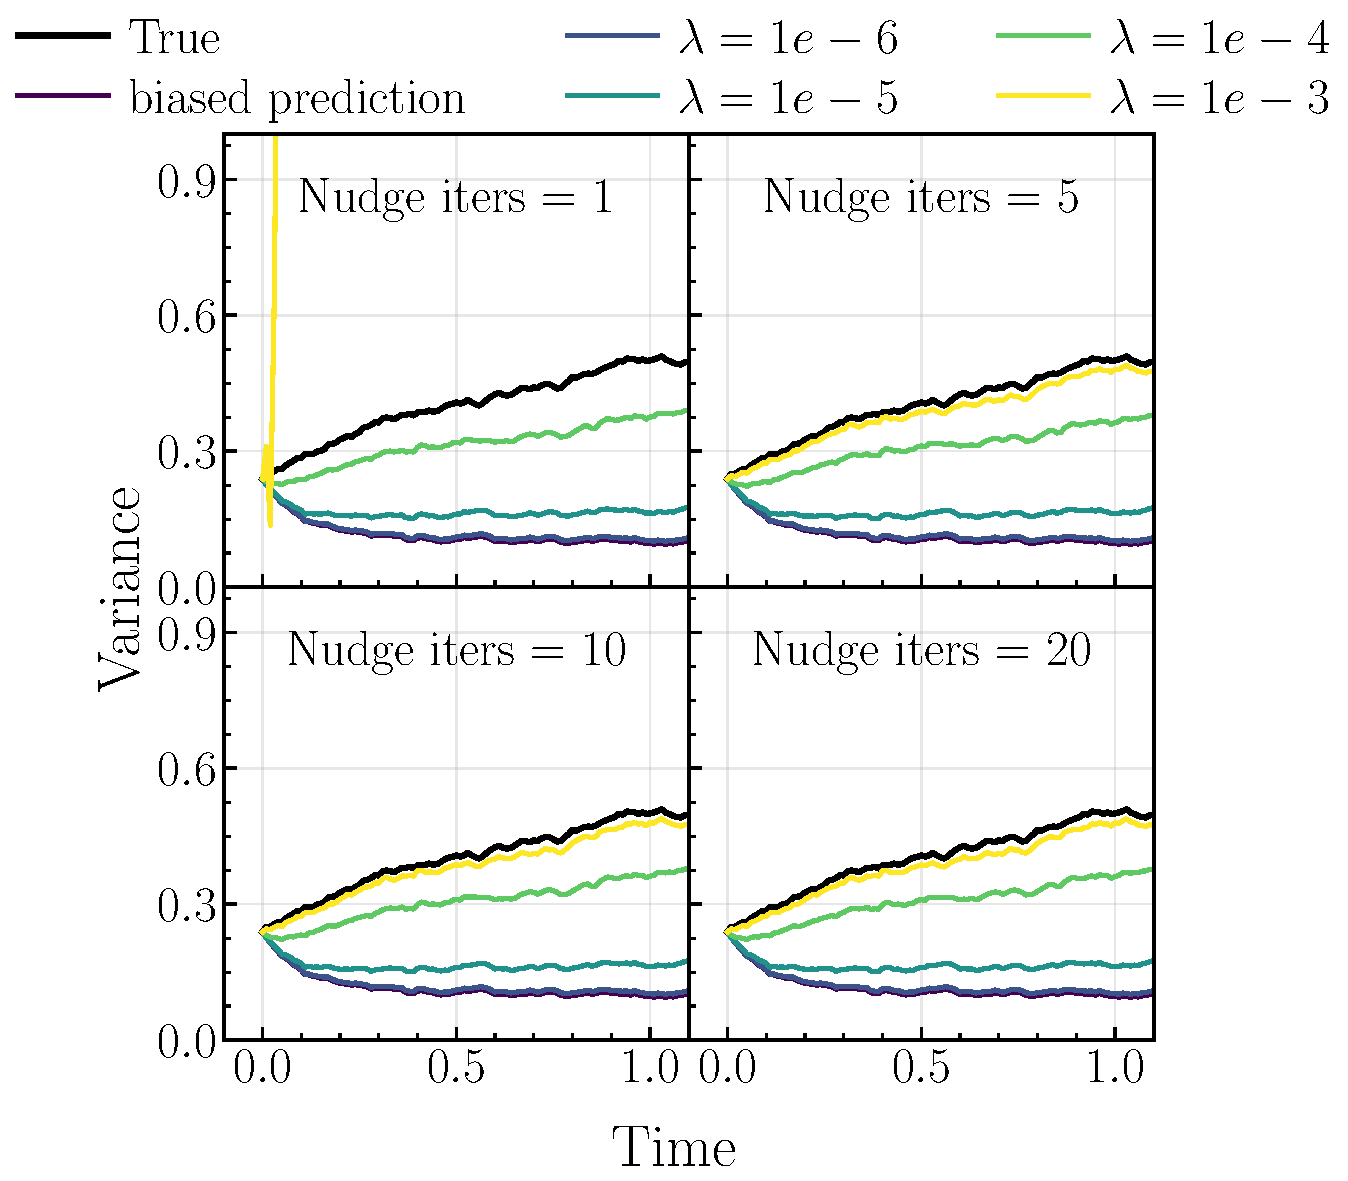
\includegraphics[width=0.8\textwidth]{../figure/1d_case_a_0.5.pdf}
    \caption{\textbf{Variance dynamics in the one-dimensional linear benchmark (\(a=0.5\)).} We compare the reference system, the biased forecast model, and assimilated (nudged) trajectories with \(\lambda\in\{10^{-6},10^{-5},10^{-4},10^{-3}\}\). The four panels correspond to different numbers of nudging iterations. Increasing \(\lambda\) improves tracking accuracy, while excessively large nudging can introduce transient numerical instability when the correction is applied too aggressively.}
    \label{fig:simple_linear_case_a_0.5}
\end{figure}

To move beyond a single moment diagnostic, Figure~\ref{fig:simple_linear_case_density_a_0.5} compares the full space--time density for the true dynamics, the biased forecast, and two assimilated solutions. The biased model is overly diffuse and fails to reproduce the concentration near \(x=0\). A moderate correction (\(\lambda=10^{-5}\)) partially restores the correct density profile, while the stronger correction (\(\lambda=10^{-3}\)) yields a space--time distribution much closer to the reference one. This confirms that the nudging term corrects the full law rather than merely matching low-order statistics.

\begin{figure}[h]
    \centering
    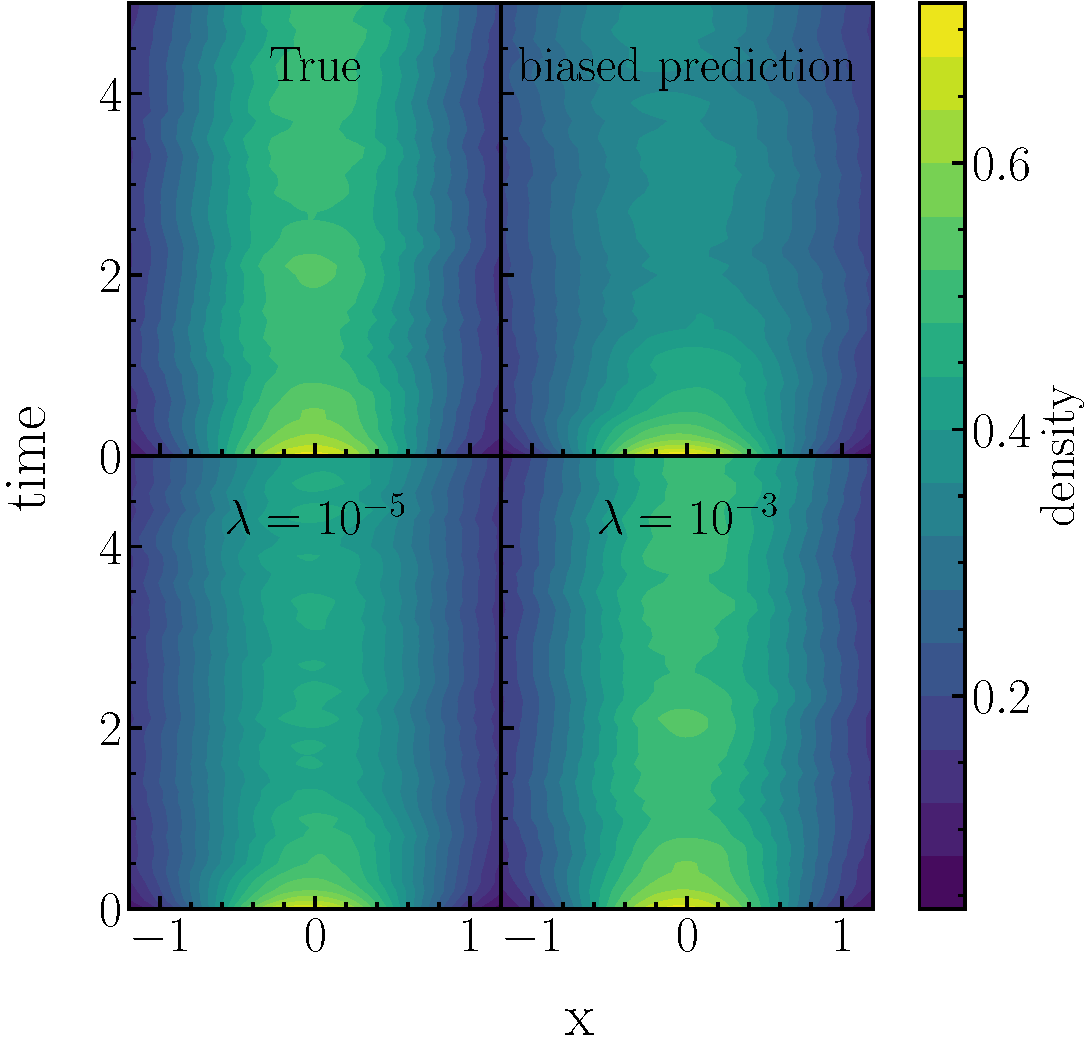
\includegraphics[width=0.8\textwidth]{../figure/1d_case_density_a_0.5.pdf}
    \caption{\textbf{Space--time density evolution in the linear benchmark (\(a=0.5\)).} Top-left: reference density. Top-right: biased forecast. Bottom-left: assimilated density with \(\lambda=10^{-5}\). Bottom-right: assimilated density with \(\lambda=10^{-3}\). Larger nudging strength restores both the location and the spread of the true law.}
    \label{fig:simple_linear_case_density_a_0.5}
\end{figure}

Figure~\ref{fig:simple_linear_case_w2} summarizes the final-time and time-averaged \(W_2\) errors for all three biased models as functions of \(\lambda\). Both error metrics decrease nearly monotonically as the nudging strength increases, with the most visible gains occurring between \(10^{-5}\) and \(10^{-3}\). The reduction is consistent across both under-interacting and over-interacting forecast models, which supports the theoretical conclusion of Theorem~\ref{thm:main_kdenudge}: sufficiently strong observation feedback suppresses the error induced by model misspecification.

\begin{figure}
    \centering
    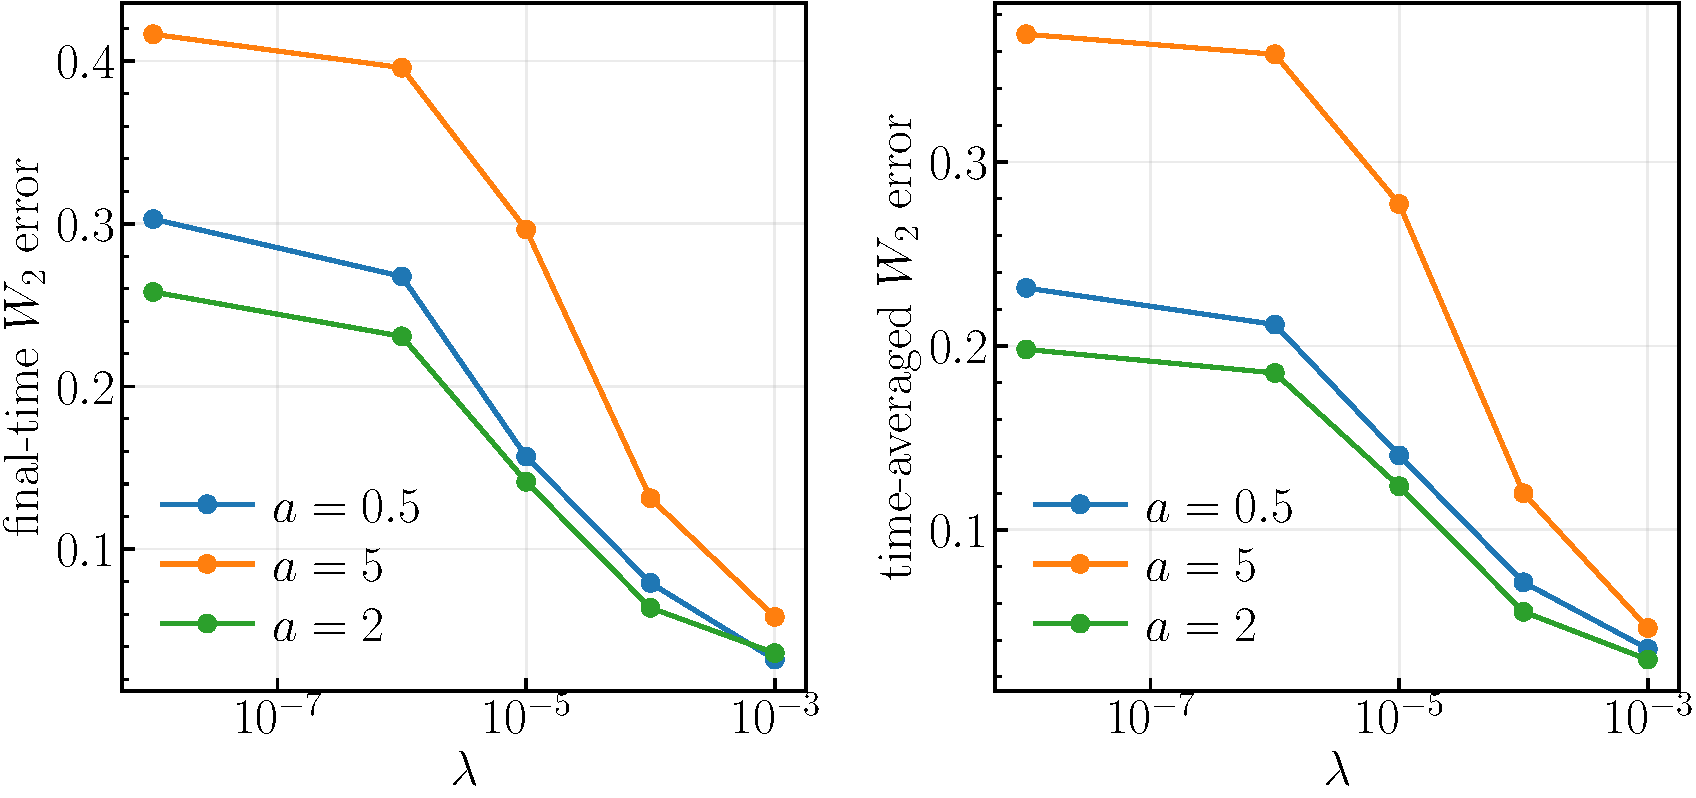
\includegraphics[width=0.8\linewidth]{figure/w2_vs_lambda_iter20.pdf}
    \caption{\textbf{Distributional error versus nudging strength in the linear benchmark.} Left: final-time \(W_2\) error. Right: time-averaged \(W_2\) error. In all three biased models \(a\in\{0.5,2,5\}\), stronger nudging produces a smaller distributional discrepancy with the reference dynamics.}
    \label{fig:simple_linear_case_w2}
\end{figure}


\subsection{Multimodal distribution}

We next consider a one-dimensional interacting particle system with a bistable confining potential,
\begin{equation}
    \intd X_t^i = -\nabla U(X_t^i)\,\intd t -a\bigl(X_t^i - m_t\bigr)\,\intd t + \intd W_t^i,
\end{equation}
where
\[
U(x) = \frac{x^4}{4} -\frac{x^2}{2}, 
\quad
m_t = \frac{1}{N}\sum_{i=1}^N X_t^i
\]
is the empirical mean. As \(N \to \infty\), the associated mean-field limit is given by
\[
\intd \bar X_t = - (\bar{X}_t^3 - \bar{X}_t )\,\intd t -a\bigl(\bar X_t - \bar m_t\bigr)\,\intd t + \intd W_t,
\qquad
\bar m_t = \int x\,\mu_t(\intd x),
\]
where \(\mu_t = \mathrm{Law}(\bar X_t)\). The corresponding Fokker--Planck equation reads
\[
\partial_t \mu_t
= \partial_x\!\left( (x^3-x )\mu_t\right)
+ \partial_x\!\left( a\left(x-\int x\,\mu_t(\intd x)\right)\mu_t\right)
+ \frac{1}{2}\partial_{xx}\mu_t.
\]

This benchmark is substantially more challenging than the linear Gaussian case because the double-well potential generates a genuinely bimodal law with metastable transitions between the two wells. In this regime, matching only the mean or the variance is insufficient: two distributions can have similar low-order moments while placing mass in the wrong well. We therefore use this example to test whether the kernel-based nudging term can transfer probability mass across the barrier at \(x=0\), recover the correct modal locations, and preserve the relative weights of the two modes from smoothed macroscopic observations. In the experiments, we again generate the reference data with the true interaction coefficient $a=0.25$ and initial position $X^i_0 \sim \mathcal{N}(0,0.5)$ and integrate the particle system using Euler-Maruyama with time step $t=0.01$ up to final time $T=5$. As before, observations are generated from the smoothed density $K_h*\mu_t$ with $h=0.5$, and the forecast model is  misspecified through the interaction coefficient \(a\) with $a\in\{0.1,0.5,1.5\}$. The quality of assimilation is evaluated through density snapshots together with the corresponding Wasserstein error. This example highlights that the proposed correction mechanism is not restricted to unimodal or near-Gaussian laws.

\begin{figure}[htbp]
    \centering
    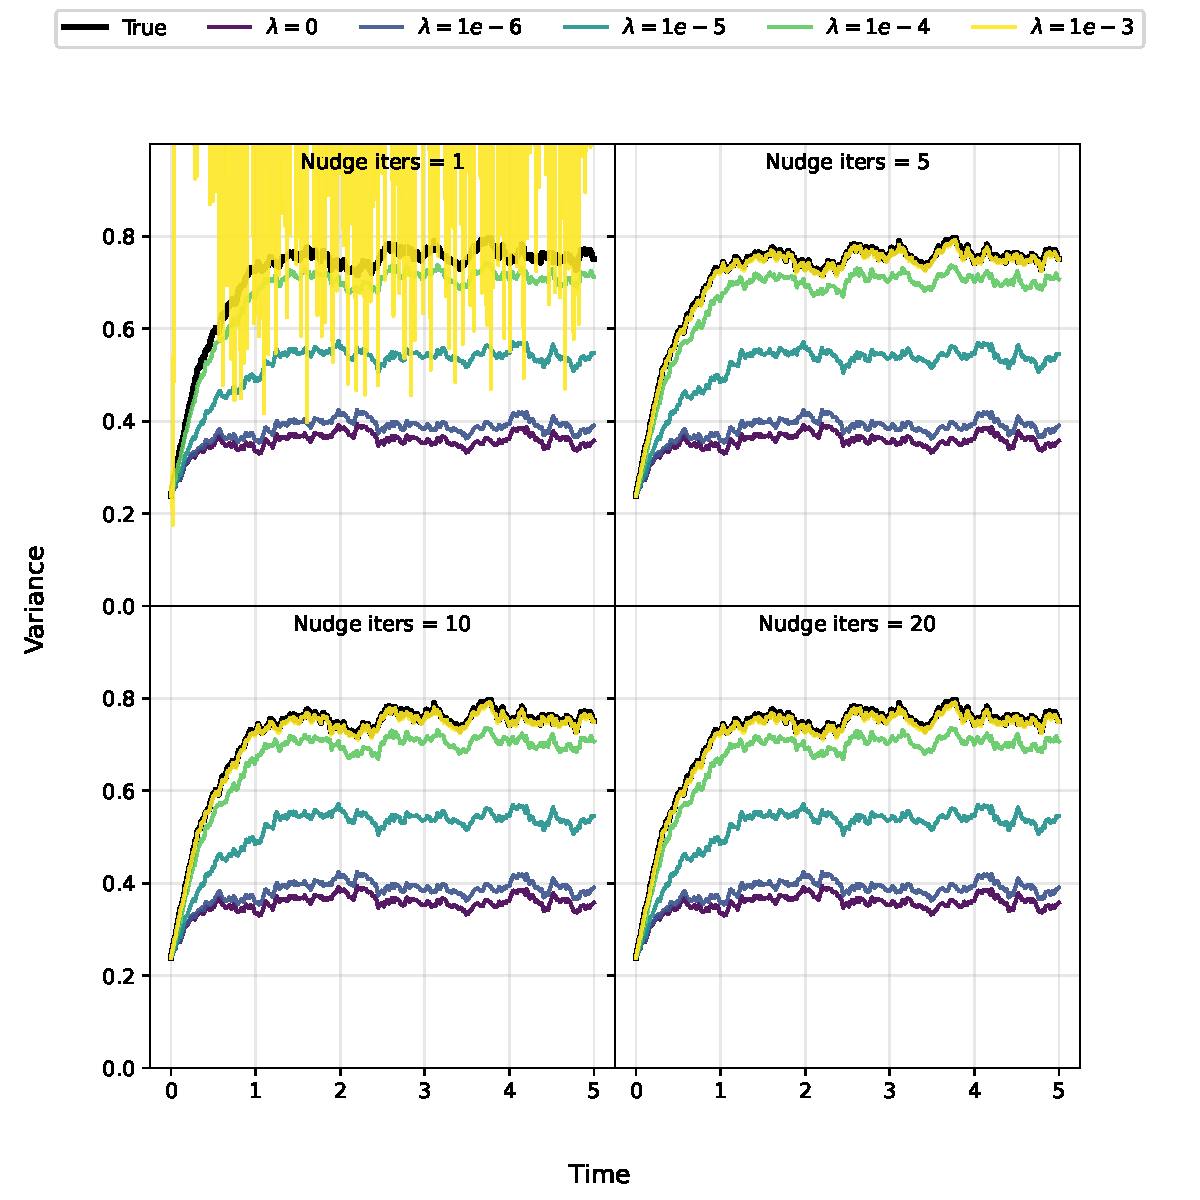
\includegraphics[width=0.8\textwidth]{../figure/case2_true_0.25_a_1.5.pdf}
    \caption{\textbf{Variance dynamics in the multimodal benchmark (\(a=1.5\)).} We compare the reference system, the biased forecast model, and assimilated (nudged) trajectories with \(\lambda\in\{10^{-6},10^{-5},10^{-4},10^{-3}\}\). The four panels correspond to different numbers of nudging iterations. Increasing \(\lambda\) improves tracking accuracy, while excessively large nudging can introduce transient numerical instability when the correction is applied too aggressively.}
    \label{fig:case2_true_0.25_a_1.5}
\end{figure}

Figure \ref{fig:case2_true_0.25_a_1.5} shows the variance dynamics for $a=1.5$ for four different nudging iterations. The biased forecast model performs worse than all the assimilated forecast models. After enough nudging iterations, the assimilated model with nudging intensity $\lambda = 10^{-3}$ produces the closest approximation to the reference solution, but with just one nudging iteration, the model overestimates the variance and generates high oscillations, which is to be expected due to the tradeoff between accuracy and stability.

\begin{figure}[h]
    \centering
    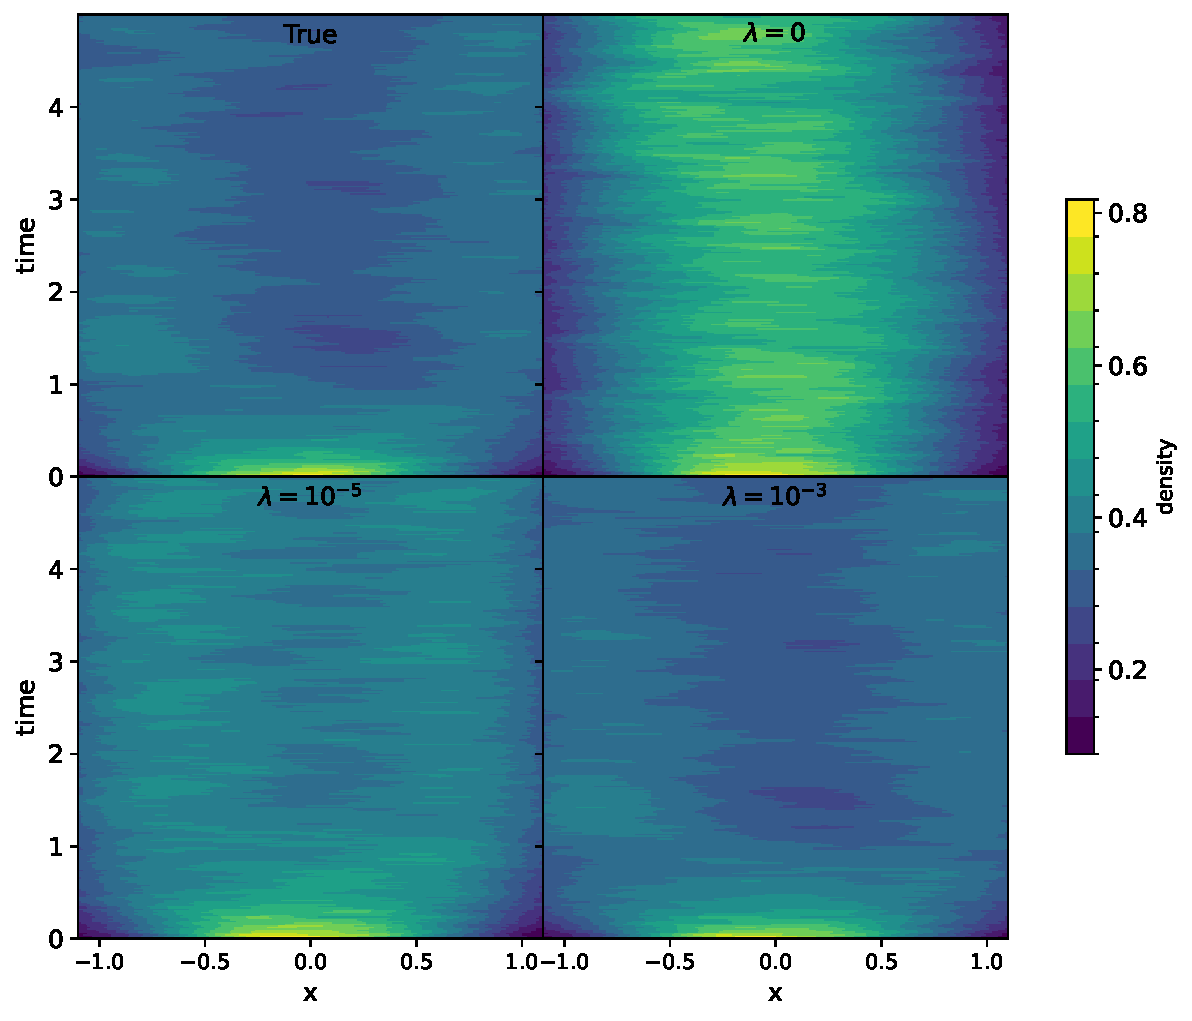
\includegraphics[width=0.8\textwidth]{../figure/case2_density_true_0.25_a_1.5.pdf}
    \caption{\textbf{Space--time density evolution in the multimodal benchmark (\(a=1.5\)).} Top-left: reference density. Top-right: biased forecast. Bottom-left: assimilated density with \(\lambda=10^{-5}\). Bottom-right: assimilated density with \(\lambda=10^{-3}\). Larger nudging strength restores both the location and the spread of the true law.}
    \label{fig:case2_density_true_0.25_a_1.5}
\end{figure}

In Figure \ref{fig:case2_density_true_0.25_a_1.5}, the space-time densities for the true reference solution, biased prediction, and two assimilated forecasts with $a=1.5$ are shown. The prediction from the biased model is overly concentrated around $x=0$ and does not capture the density profile of the true solution, which has two high probability regions. The assimilated model with $\lambda = 10^{-5}$ moderately diffuses the concentration near $x=0$ and partially shows the two modes, whereas the model with $\lambda = 10^{-3}$ achieves the closest match to the reference density and clearly shows the two stable regions of high probability.

\begin{figure}
    \centering
    \begin{subfigure}[t]{0.45\linewidth}\centering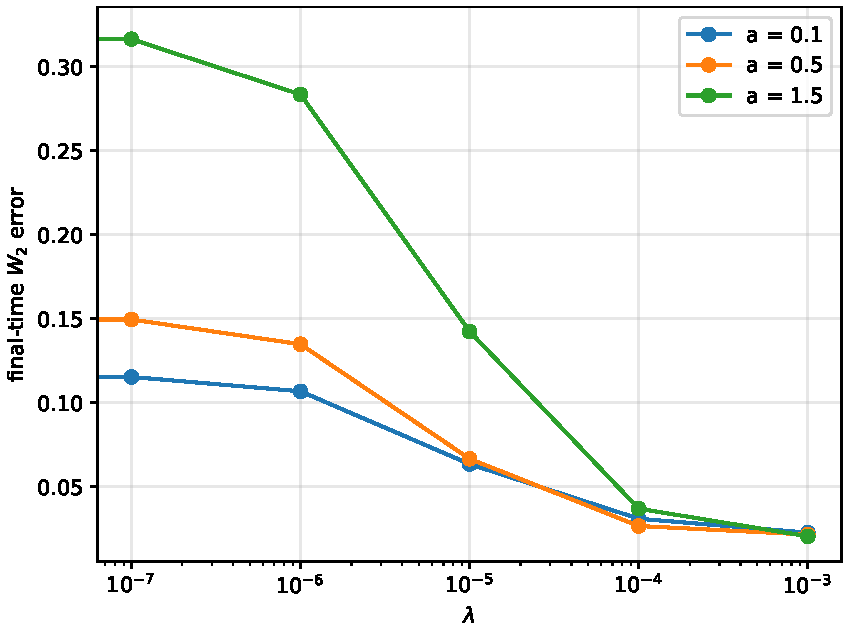
\includegraphics[width=\linewidth]{../figure/case2_true_0.25_finaltime_w2.pdf}
    \end{subfigure}
    \begin{subfigure}[t]{0.45\linewidth}\centering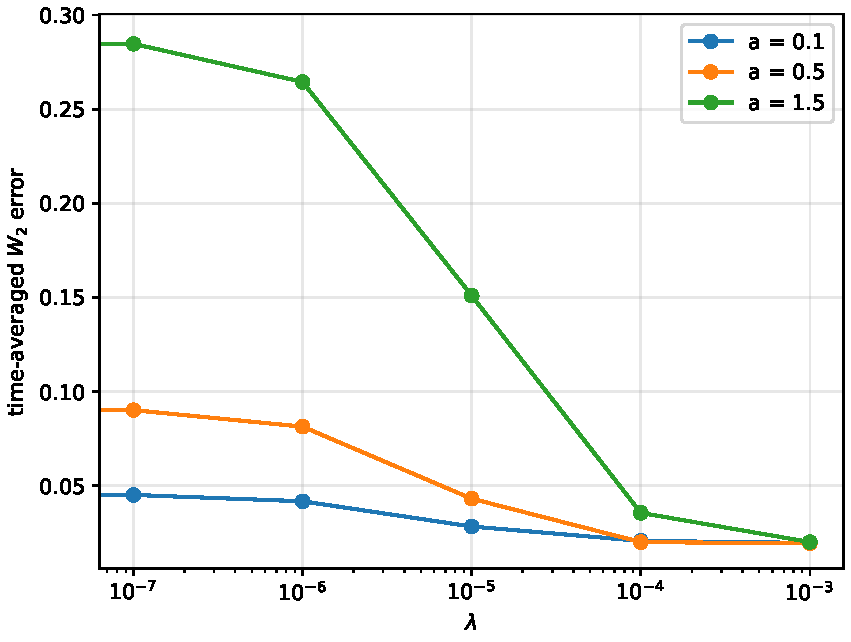
\includegraphics[width=\linewidth]{../figure/case2_true_0.25_timeavg_w2.pdf}
    \end{subfigure}
    \caption{\textbf{Distributional error versus nudging strength in the multimodal benchmark.} Left: final-time \(W_2\) error. Right: time-averaged \(W_2\) error. In all three biased models \(a\in\{0.1,0.5,1.5\}\), stronger nudging produces a smaller distributional discrepancy with the reference dynamics.}
    \label{fig:case2_true_0.25_w2}
\end{figure}

Figure \ref{fig:case2_true_0.25_w2} displays the final-time and time-averaged $W_2$ errors for the forecast models with $a\in \{0.1,0.5,1.5\}$ as functions of the nudging intensity $\lambda$. As $\lambda$ increases, both errors decrease monotonically across all three biased models, which is consistent with the conclusion of Theorem~\ref{thm:main_kdenudge}.

\subsection{Lorenz dynamics}

We further consider a mean-field Lorenz system
\[
\begin{aligned}
          \intd X^i_t =& \sigma (m_{t,y} - X^i_t)\,\intd t + \sigma \,\intd W_t^{x,1},\\
         \intd Y^i_t =& [m_{t,x} (\rho - m_{t,z}) - Y^i_t]\,\intd t + \sigma \,\intd W_t^{y,1},\\
         \intd Z^i_t =& [m_{t,x} m_{t,y} - \beta Z^i_t]\,\intd t + \sigma \,\intd W_t^{z,1},   
\end{aligned}
\]
where \(m_{t,x}\), \(m_{t,y}\), and \(m_{t,z}\) denote the empirical means of the three coordinates. As a biased forecast model, we use \(N\) individual Lorenz systems without the mean-field coupling,
\[
\begin{aligned}
          \intd X^i_t =& \sigma (Y^i_t - X^i_t)\,\intd t + \sigma \,\intd W_t^{x,1},\\
         \intd Y^i_t =& [X^i_t  (\rho - Z^i_t) - Y^i_t]\,\intd t + \sigma \,\intd W_t^{y,1},\\
         \intd Z^i_t =& [X^i_t  Y^i_t - \beta Z^i_t]\,\intd t + \sigma \,\intd W_t^{z,1}.   
\end{aligned}
\]

This example probes a strongly nonlinear and chaotic regime in which small modeling errors amplify rapidly. Figure~\ref{fig:lorenz} compares the mean trajectory \((m_{t,x},m_{t,y},m_{t,z})\) of the assimilated system with the reference attractor for \(\lambda\in\{10^{-3},10^{-4},10^{-5}\}\). When \(\lambda=10^{-3}\), the corrected trajectory remains close to the true attractor and the mean error stays uniformly small. For \(\lambda=10^{-4}\), the dynamics still capture the correct global structure, but a visible phase discrepancy remains. When \(\lambda=10^{-5}\), the correction is too weak and the bottom panel shows repeated spikes in the mean-trajectory error, corresponding to intermittent departures from the correct lobe of the attractor. These results show that density-level feedback can stabilize a biased microscopic forecast even in a chaotic setting.

\begin{figure}
    \centering
    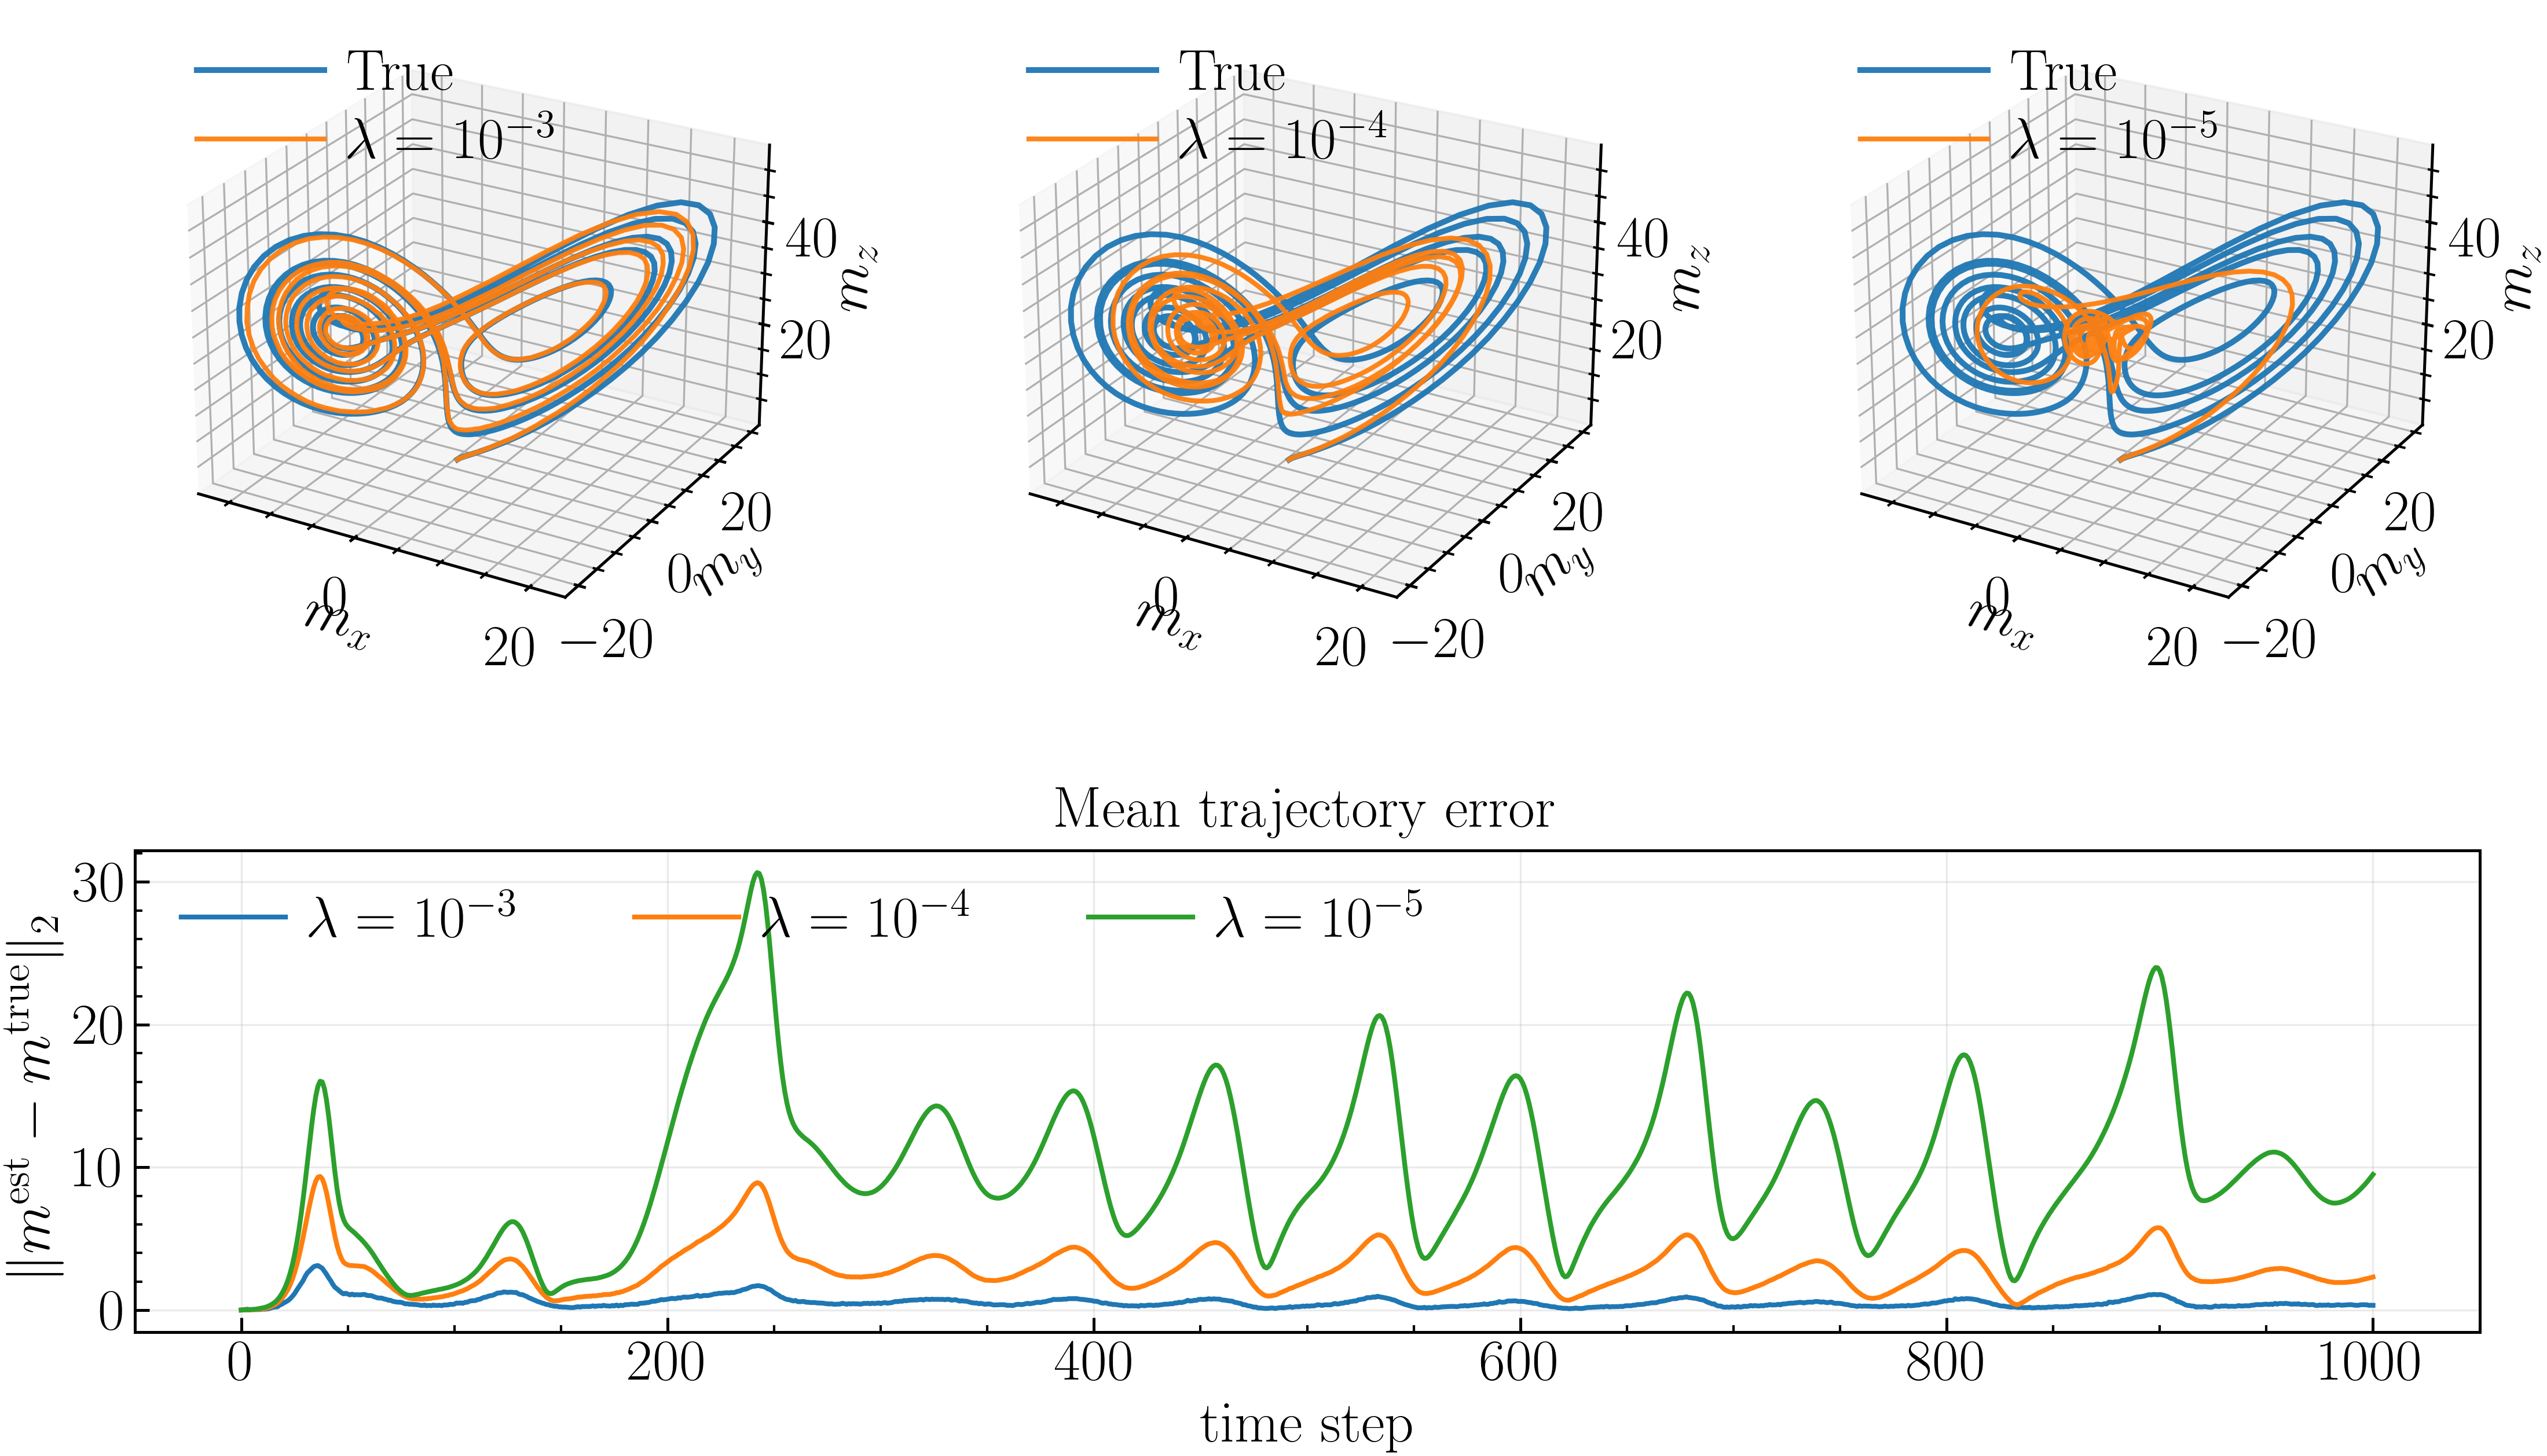
\includegraphics[width=0.9\linewidth]{figure/lorenz_lambda_comparison.png}
    \caption{\textbf{Mean-field Lorenz benchmark.} Top: trajectories of the mean state \((m_{t,x},m_{t,y},m_{t,z})\) for \(\lambda=10^{-3},10^{-4},10^{-5}\) compared with the reference attractor. Bottom: time series of the mean-trajectory error. Stronger nudging keeps the corrected dynamics close to the true attractor and suppresses intermittent excursions.}
    \label{fig:lorenz}
\end{figure}

\subsection{Vlasov--Poisson equation}

As a second example, we consider the one-dimensional Vlasov--Poisson system
\[
\begin{aligned}
    \intd X_t^i &= V_t^i \,\intd t,\\
    \intd V_t^i &= E(X_t^i,t)\,\intd t,
\end{aligned}
\]
where the self-consistent electric field is given by
\[
E(x,t) = - \nabla_x \phi(x,t),
\]
and the electrostatic potential $\phi$ solves the Poisson equation
\[
-\Delta \phi = \rho - 1, 
\qquad 
\rho(x,t) = \int f(x,v,t)\,\intd v.
\]

\paragraph{Landau damping.}
We first consider the classical Landau damping problem. The ground-truth dynamics are initialized with
\[
f(x,v,0) \propto f_{M,1}(v)\bigl(1+\varepsilon \cos(\kappa x)\bigr), 
\qquad 
f_{M,\sigma}(v) = \frac{1}{\sqrt{2\pi}\sigma}\exp\!\left(-\frac{v^2}{2\sigma^2}\right),
\]
which corresponds to a Maxwellian velocity distribution perturbed by a spatial density modulation. In our experiments, we take $\varepsilon = 0.5$ and $\kappa = \tfrac{1}{2}$.
The spatial domain is periodic with period $4\pi$, i.e., $x \in [0,4\pi]$, while the velocity domain is truncated to $v \in [-6,6]$ for numerical implementation.

To quantify the damping, we monitor the amplitude of the fundamental
Fourier mode of the electric field,
\[
E_k(t) = \left|\hat{E}(k,t)\right|,
\qquad
\hat{E}(k,t) = \frac{1}{L}\int_0^{L} E(x,t)\,e^{-ikx}\,\intd x,
\]
with $k=\kappa$ and $L=4\pi$. In the linear regime, $E_k$ decays
exponentially at the Landau damping rate.

The forecast model uses the same dynamical system but is initialized
from an unperturbed Maxwellian ($\varepsilon=0$), resulting in a biased
prediction that lacks the initial density modulation.
Figure~\ref{fig:landau_damping} compares the reference solution, the
biased forecast, and the assimilated dynamics. The results show that the
nudging term successfully reconstructs the damping behaviour and recovers
the correct exponential decay of~$E_k$.
\begin{figure}
    \centering
    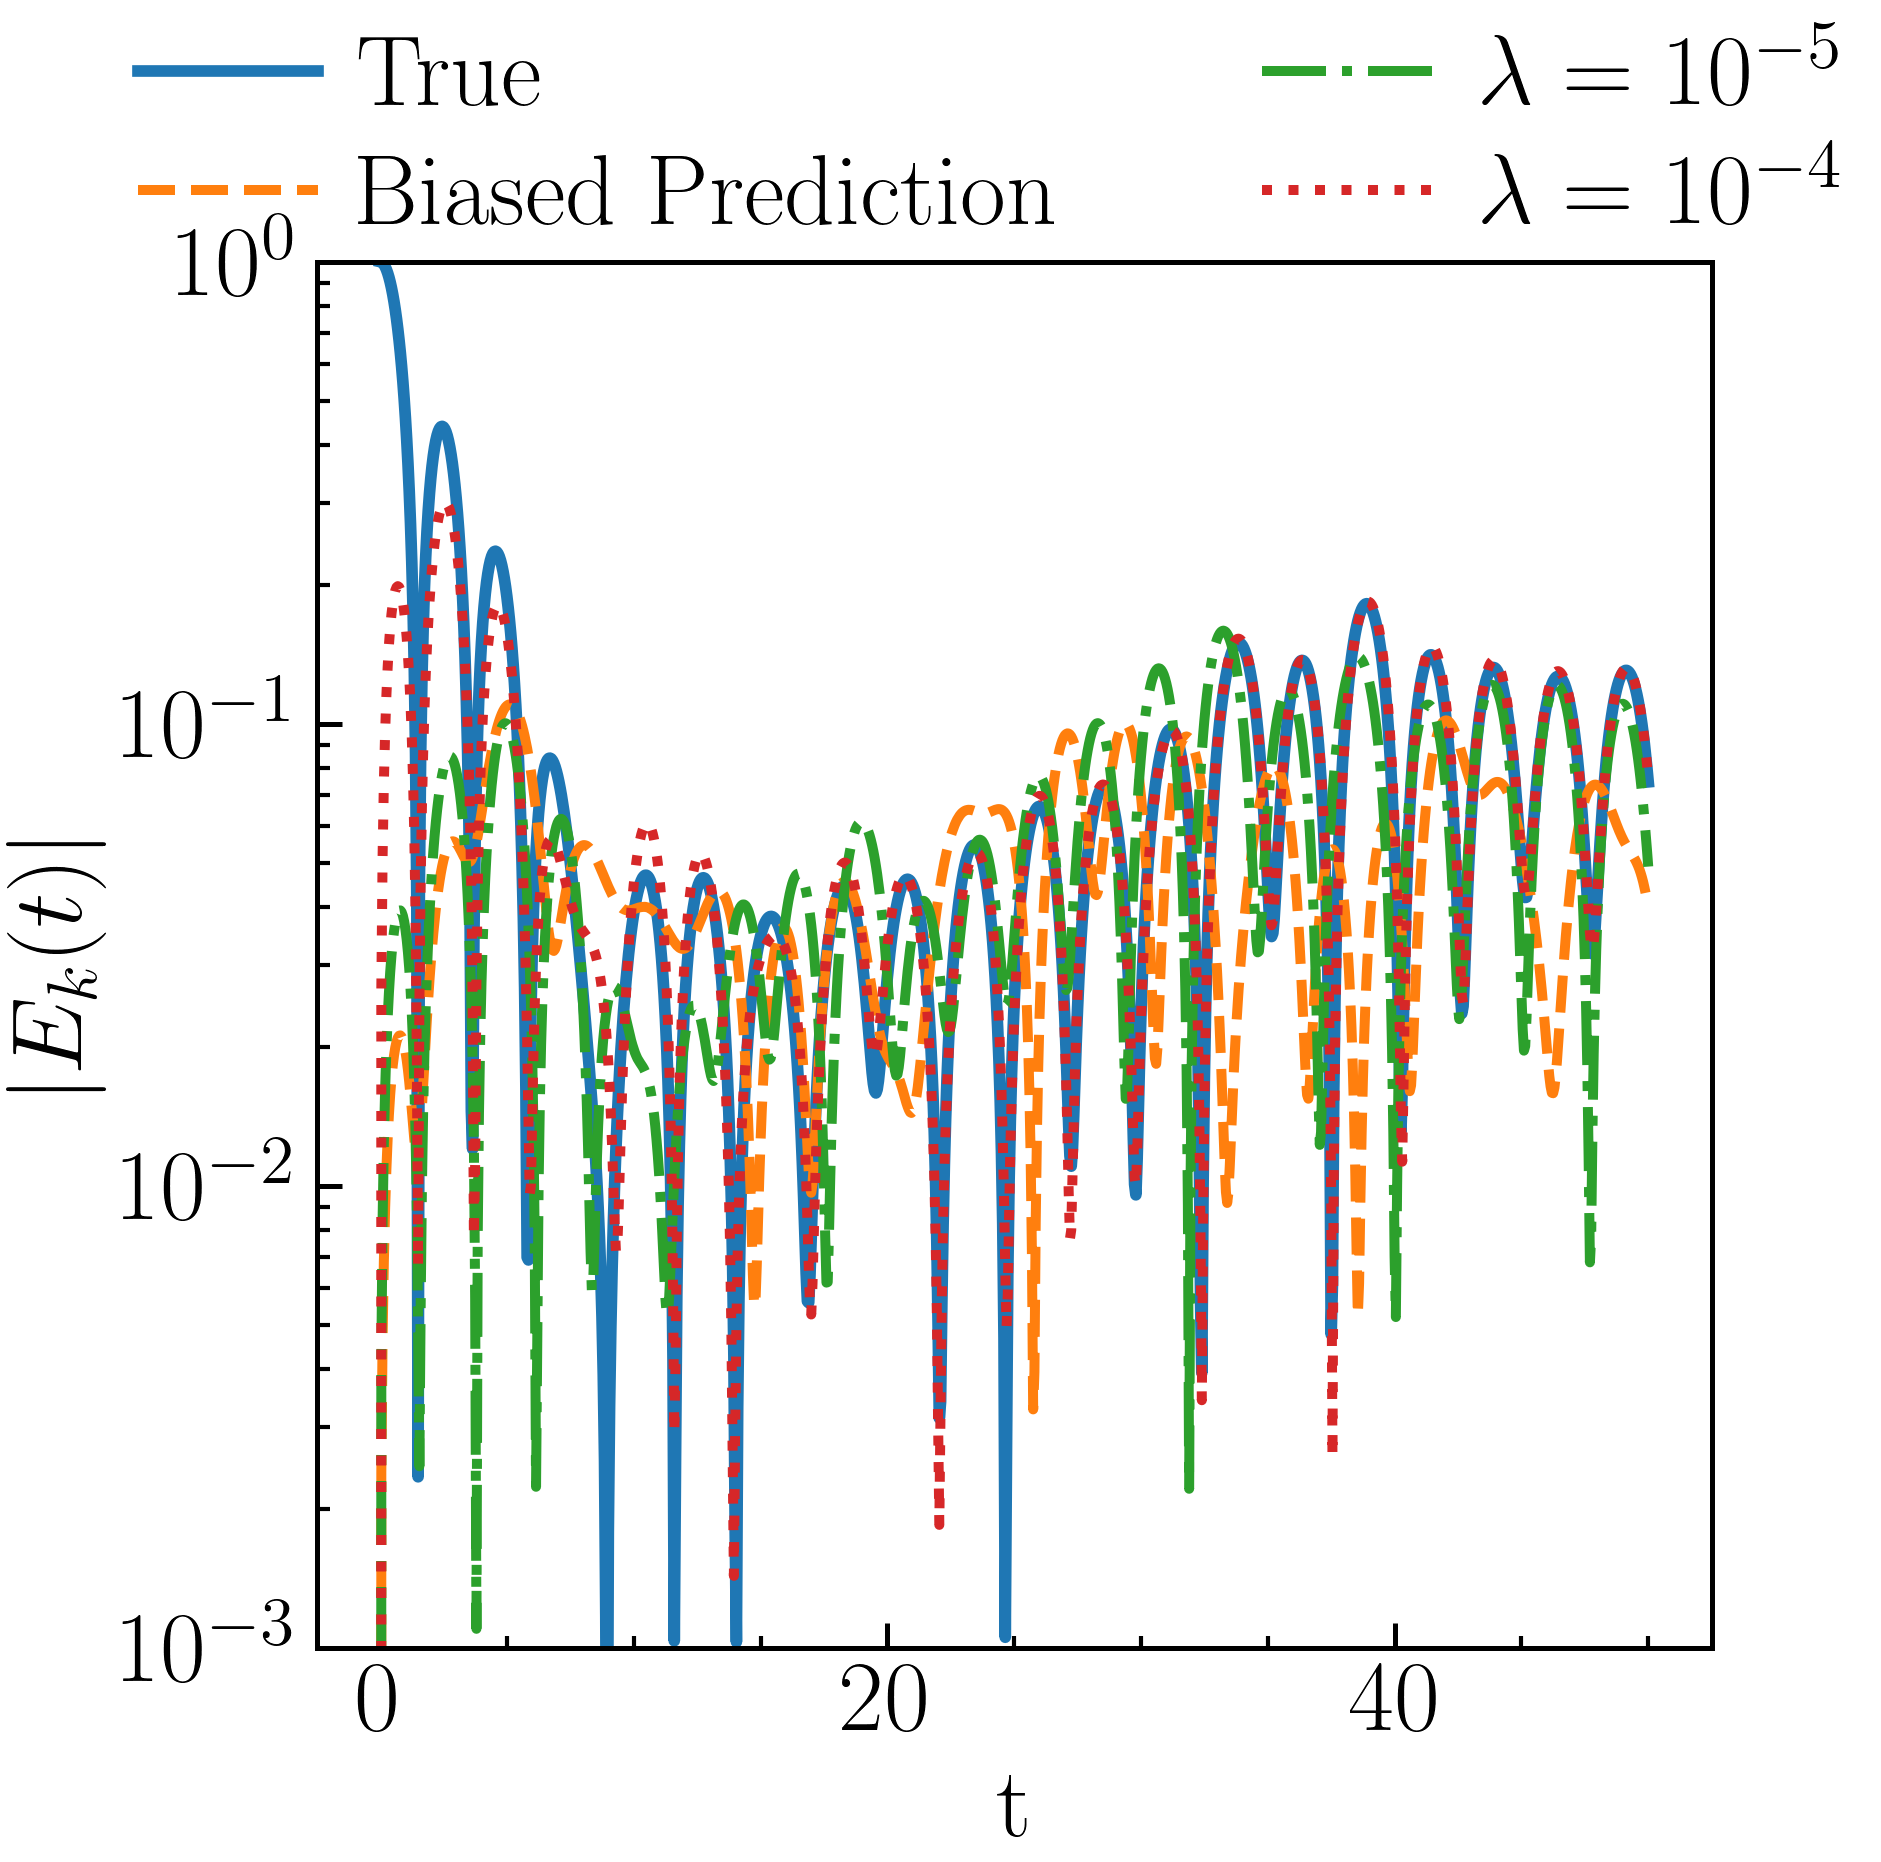
\includegraphics[width=0.5\linewidth]{figure/landau_damping.png}
    \caption{\textbf{Landau damping.} Comparison of the phase-space density
    at the final time. Left: reference solution with initial perturbation
    $\varepsilon=0.5$. Center: biased forecast initialized from the
    unperturbed Maxwellian ($\varepsilon=0$). Right: assimilated dynamics.
    The nudging term recovers the correct damping behaviour from density-level
    observations alone.}
    \label{fig:landau_damping}
\end{figure}

\paragraph{Two-stream instability.}
We next consider the two-stream instability, which exhibits strongly nonlinear behavior. The ground-truth initial condition is given by
\[
f(x,v,0) \propto \bigl(0.5 f_{M,\sigma}(v-u_0) + 0.5 f_{M,\sigma}(v+u_0)\bigr)\bigl(1+\varepsilon \cos(\kappa x)\bigr),
\]
with parameters $\sigma=0.2$, $u_0=1$, $\varepsilon=0.01$, and $\kappa=0.5$. This corresponds to a bimodal velocity distribution with a small spatial perturbation.

In contrast, the forecast model is initialized from a single Maxwellian profile,
\[
f(x,v,0) \propto f_{M,1}(v)\bigl(1+\varepsilon \cos(\kappa x)\bigr),
\]
which fails to capture the underlying two-stream structure.

Figure~\ref{fig:two_stream} shows the evolution of the system at different time steps. The biased model is unable to reproduce the filamentation and phase-space structures characteristic of the instability. In contrast, the assimilated dynamics recover the correct qualitative features, demonstrating that the proposed nudging mechanism can reconstruct nontrivial multimodal structures from macroscopic observations.

\begin{figure}
    \centering
    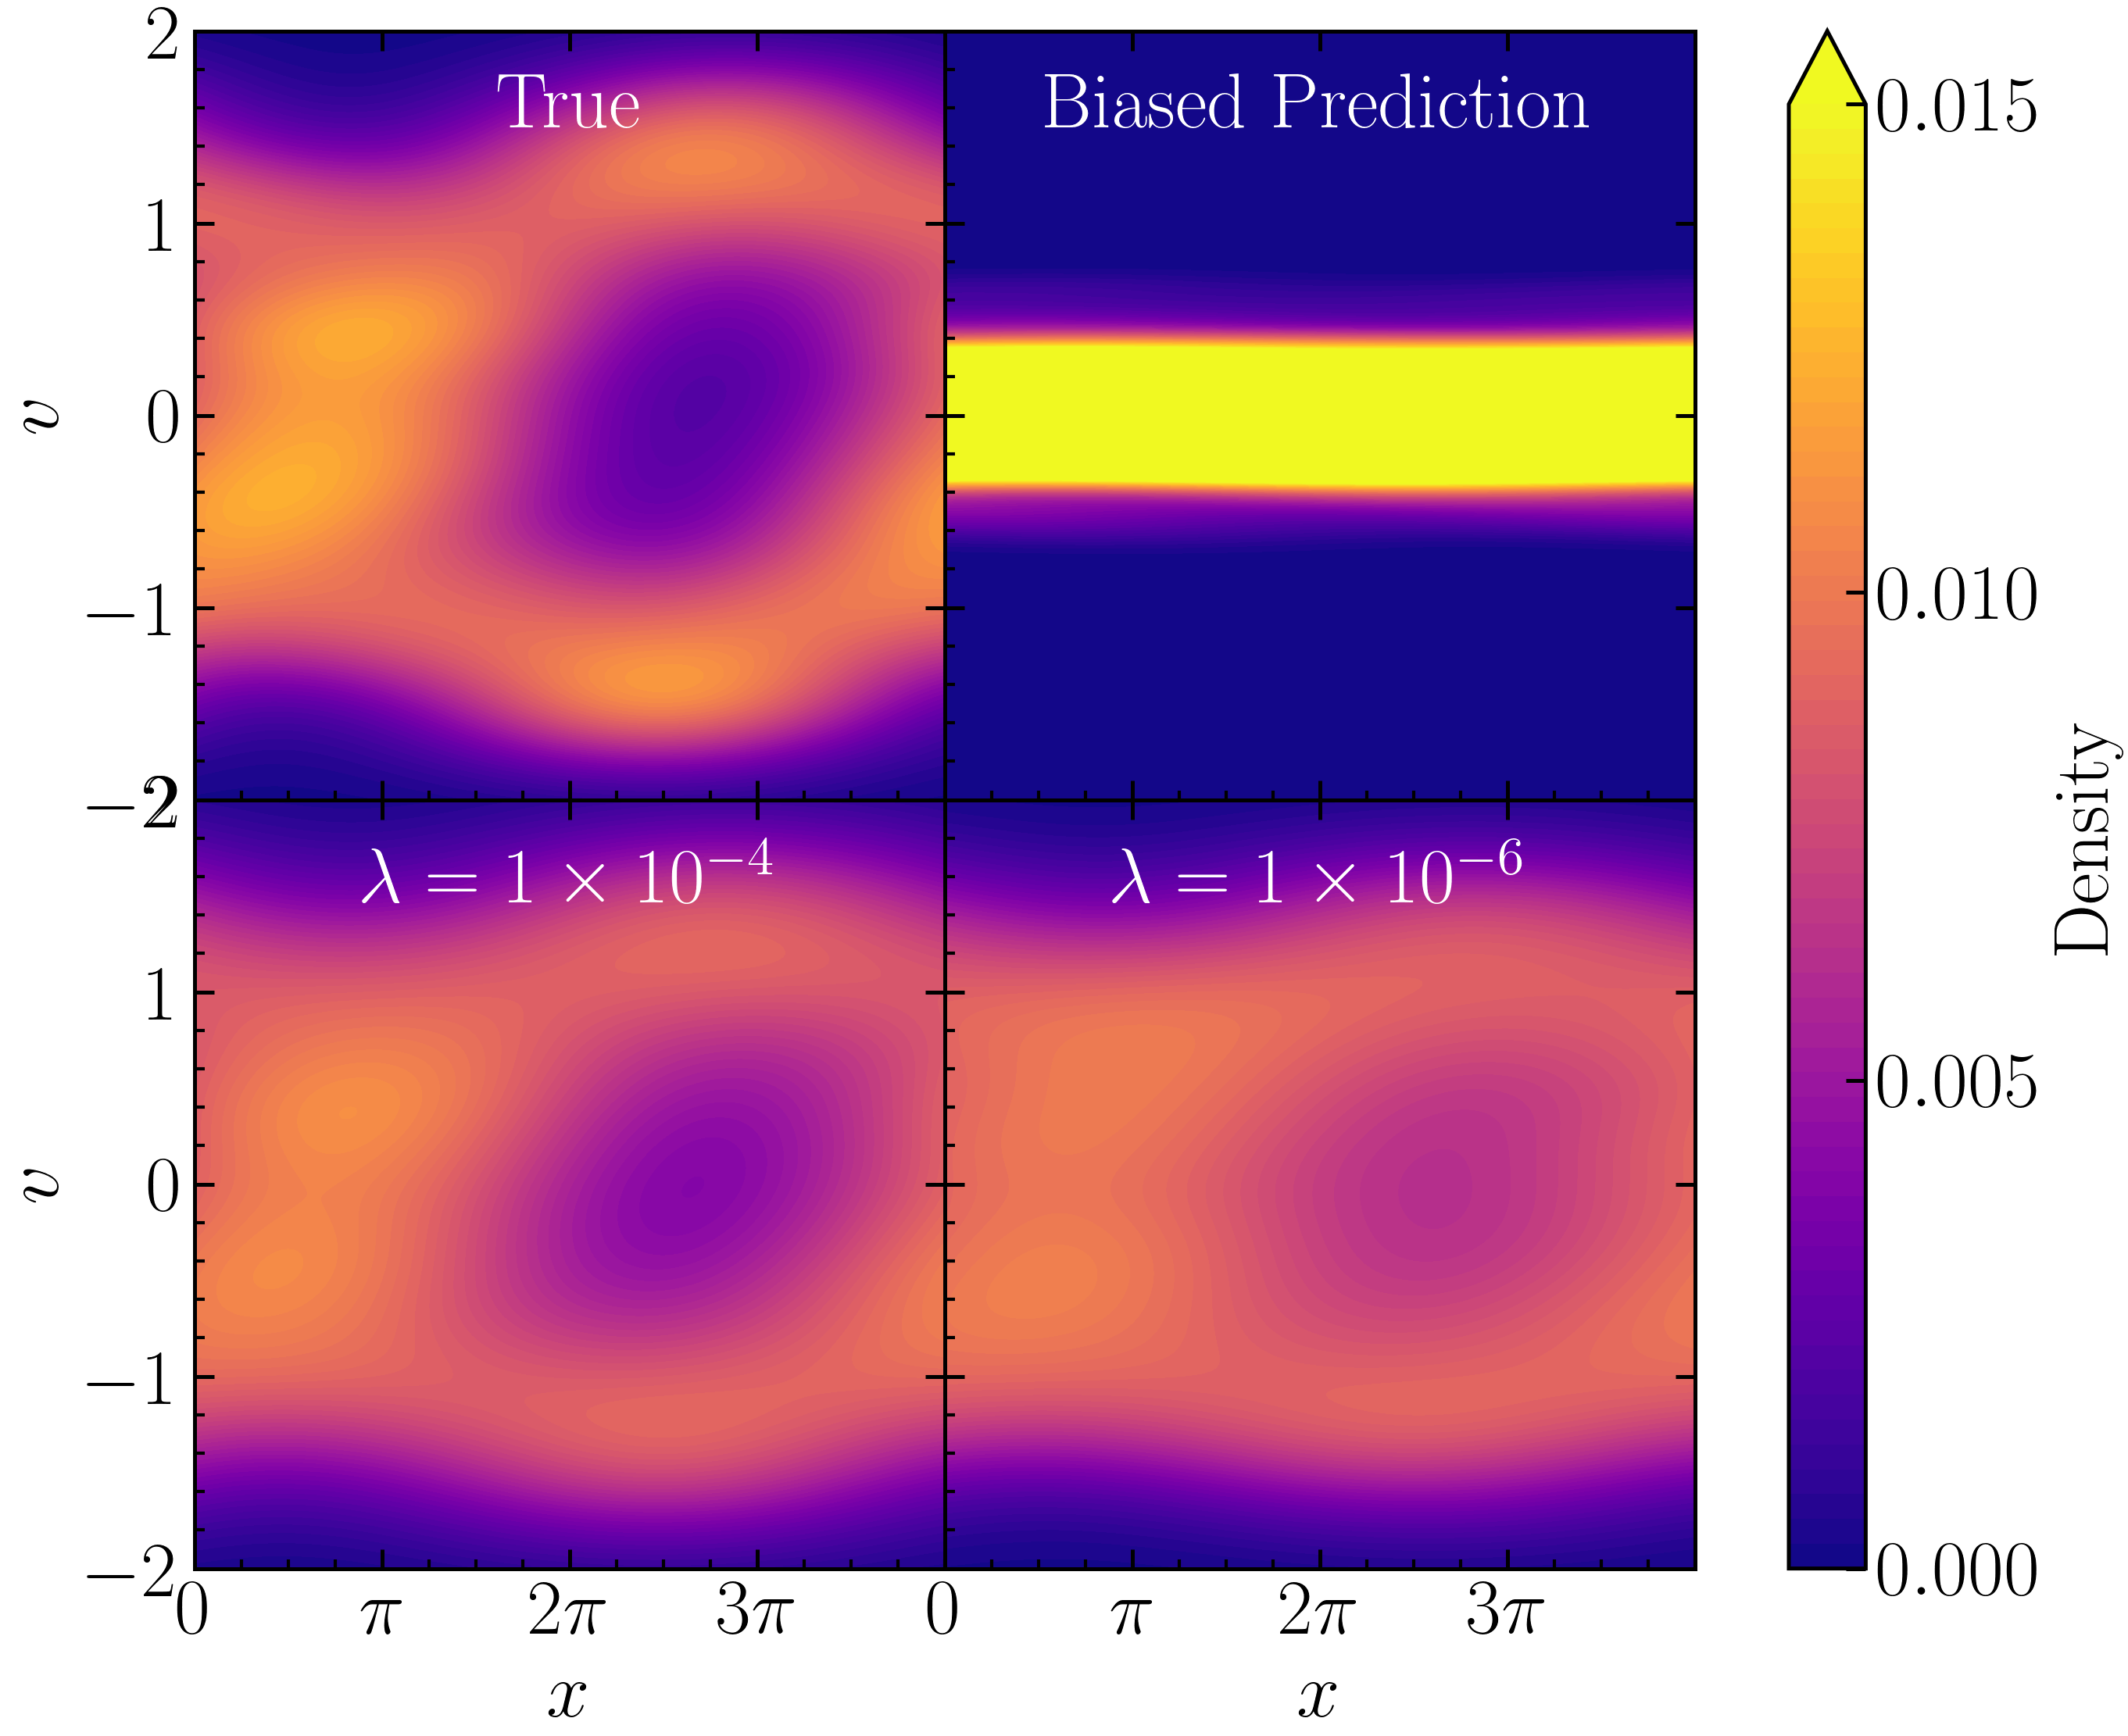
\includegraphics[width=0.49\linewidth]{figure/two_stream_step_1000.png}
    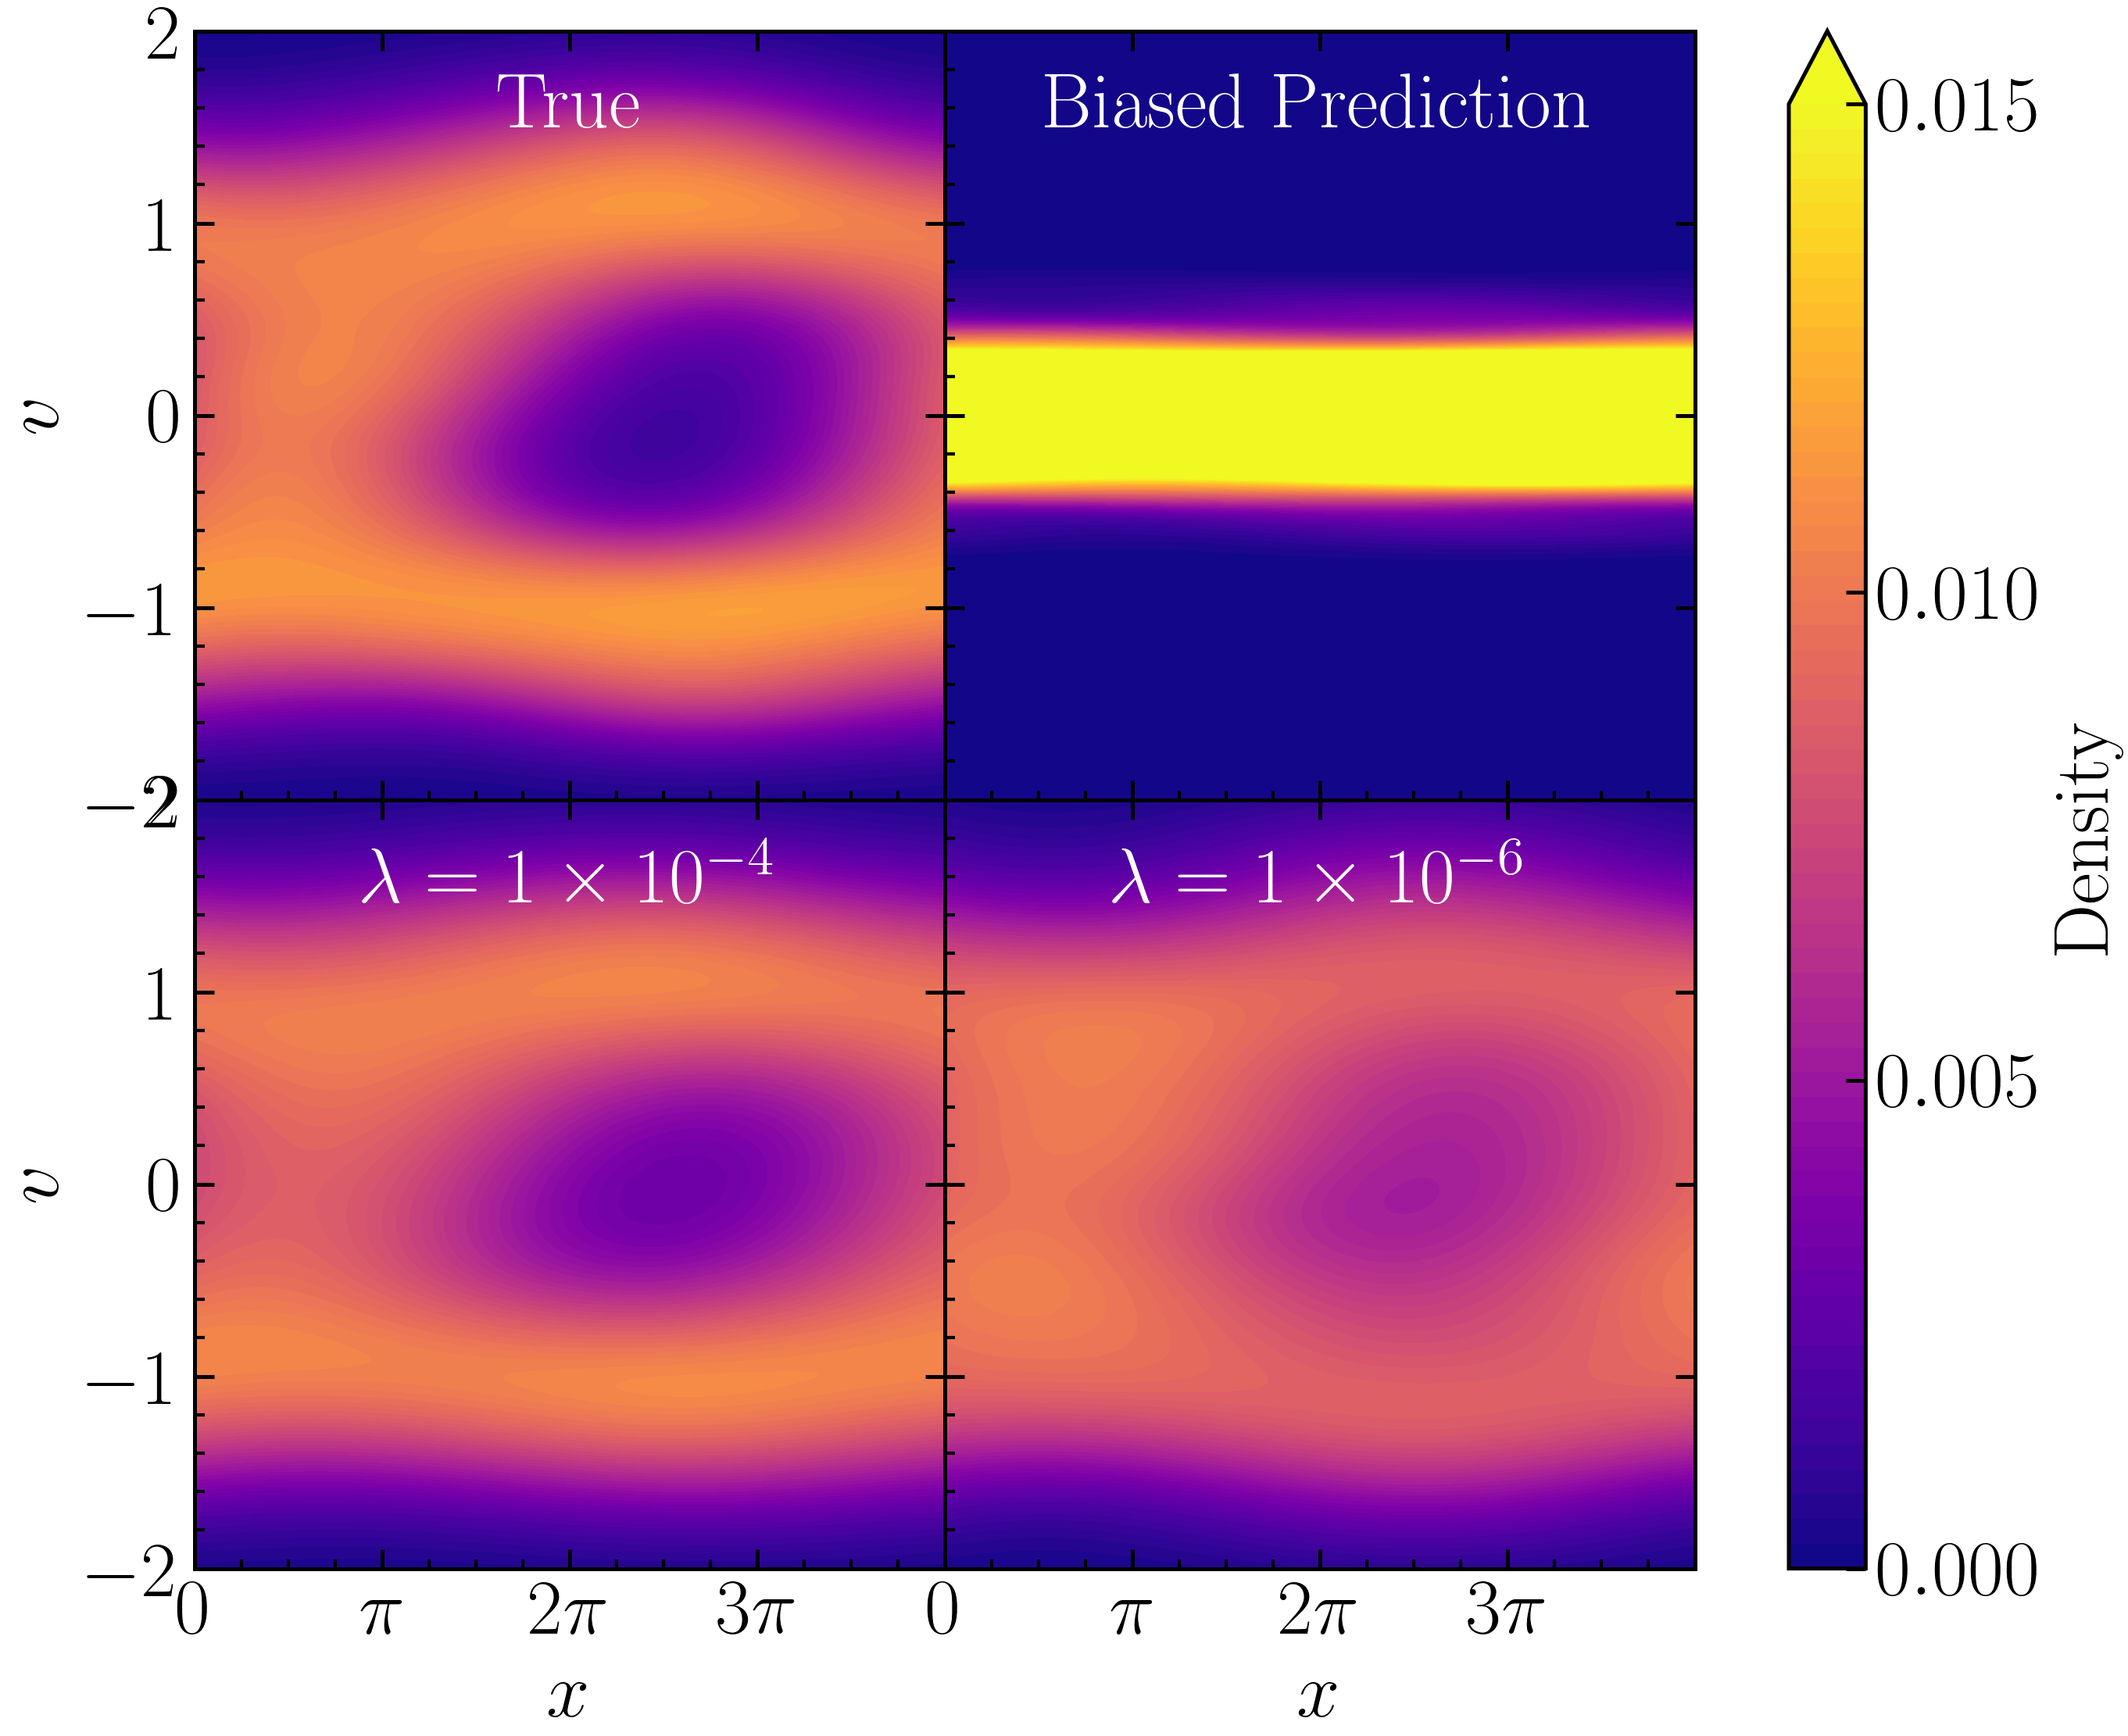
\includegraphics[width=0.49\linewidth]{figure/two_stream_step_2000.png}
    \caption{\textbf{Two-stream instability.} Phase-space density at
intermediate (left, step 1000) and late (right, step 2000) times. Each
panel compares the reference two-stream dynamics (top), the biased
single-Maxwellian forecast (center), and the assimilated solution
(bottom). The nudging recovers the filamentation and vortex-merging
structures absent from the biased model.}
\label{fig:two_stream}
\end{figure}

\subsection{Collective-motion data}

We finally apply the proposed mean-field data assimilation framework to
trajectory data obtained from experiments with approximately
\(N \approx 1000\) fish swimming in a quasi-two-dimensional
tank~\cite{walter2021trex}. The dataset consists of discrete-time
position measurements \(\{\mathbf{X}_i(t_n)\}\) that are spatially and
temporally incomplete due to visual occlusions and tracking dropouts
inherent to the image-processing pipeline. Since exact
particle-to-particle correspondence is unreliable across frames, this
example is particularly well suited to a density-based assimilation
strategy.

The domain \(\Omega\) is discretized on a uniform grid with spatial
resolution \(\Delta x\), and the observational density is constructed by
a kernel density estimator,
\begin{equation}
    \mu^{\mathrm{obs}}(x, t_n)
    = \frac{1}{N} \sum_{i=1}^N K_h(x - X_i(t_n)),
\end{equation}
where \(K_h\) is a Gaussian smoothing kernel with bandwidth \(h\). An
approximate microscopic model is first learned by fitting a mean-field
interaction force~\cite{lyu2026mvnn} to short segments of the historical
trajectories; the proposed nudging step is then applied using the
image-based density observations.

Figure~\ref{fig:fish_t_50} shows a representative comparison at time
step~\(50\). The top row contains the raw image frame and the particle
configuration predicted by the assimilated model. The bottom row compares
the density reconstructed from image processing with the density of the
corrected particle system. The two density fields agree well at the
macroscopic level: the assimilated prediction captures the overall
ring-shaped occupancy of the tank, the dominant high-density regions in
the center-left and lower-middle part of the domain, and the low-density
boundary regions near the wall. The remaining discrepancies are localized
and do not alter the large-scale organization of the school. This
experiment shows that the framework can translate incomplete image-based
observations into a microscopic particle forecast without requiring exact
particle matching.

\begin{figure}
    \centering
    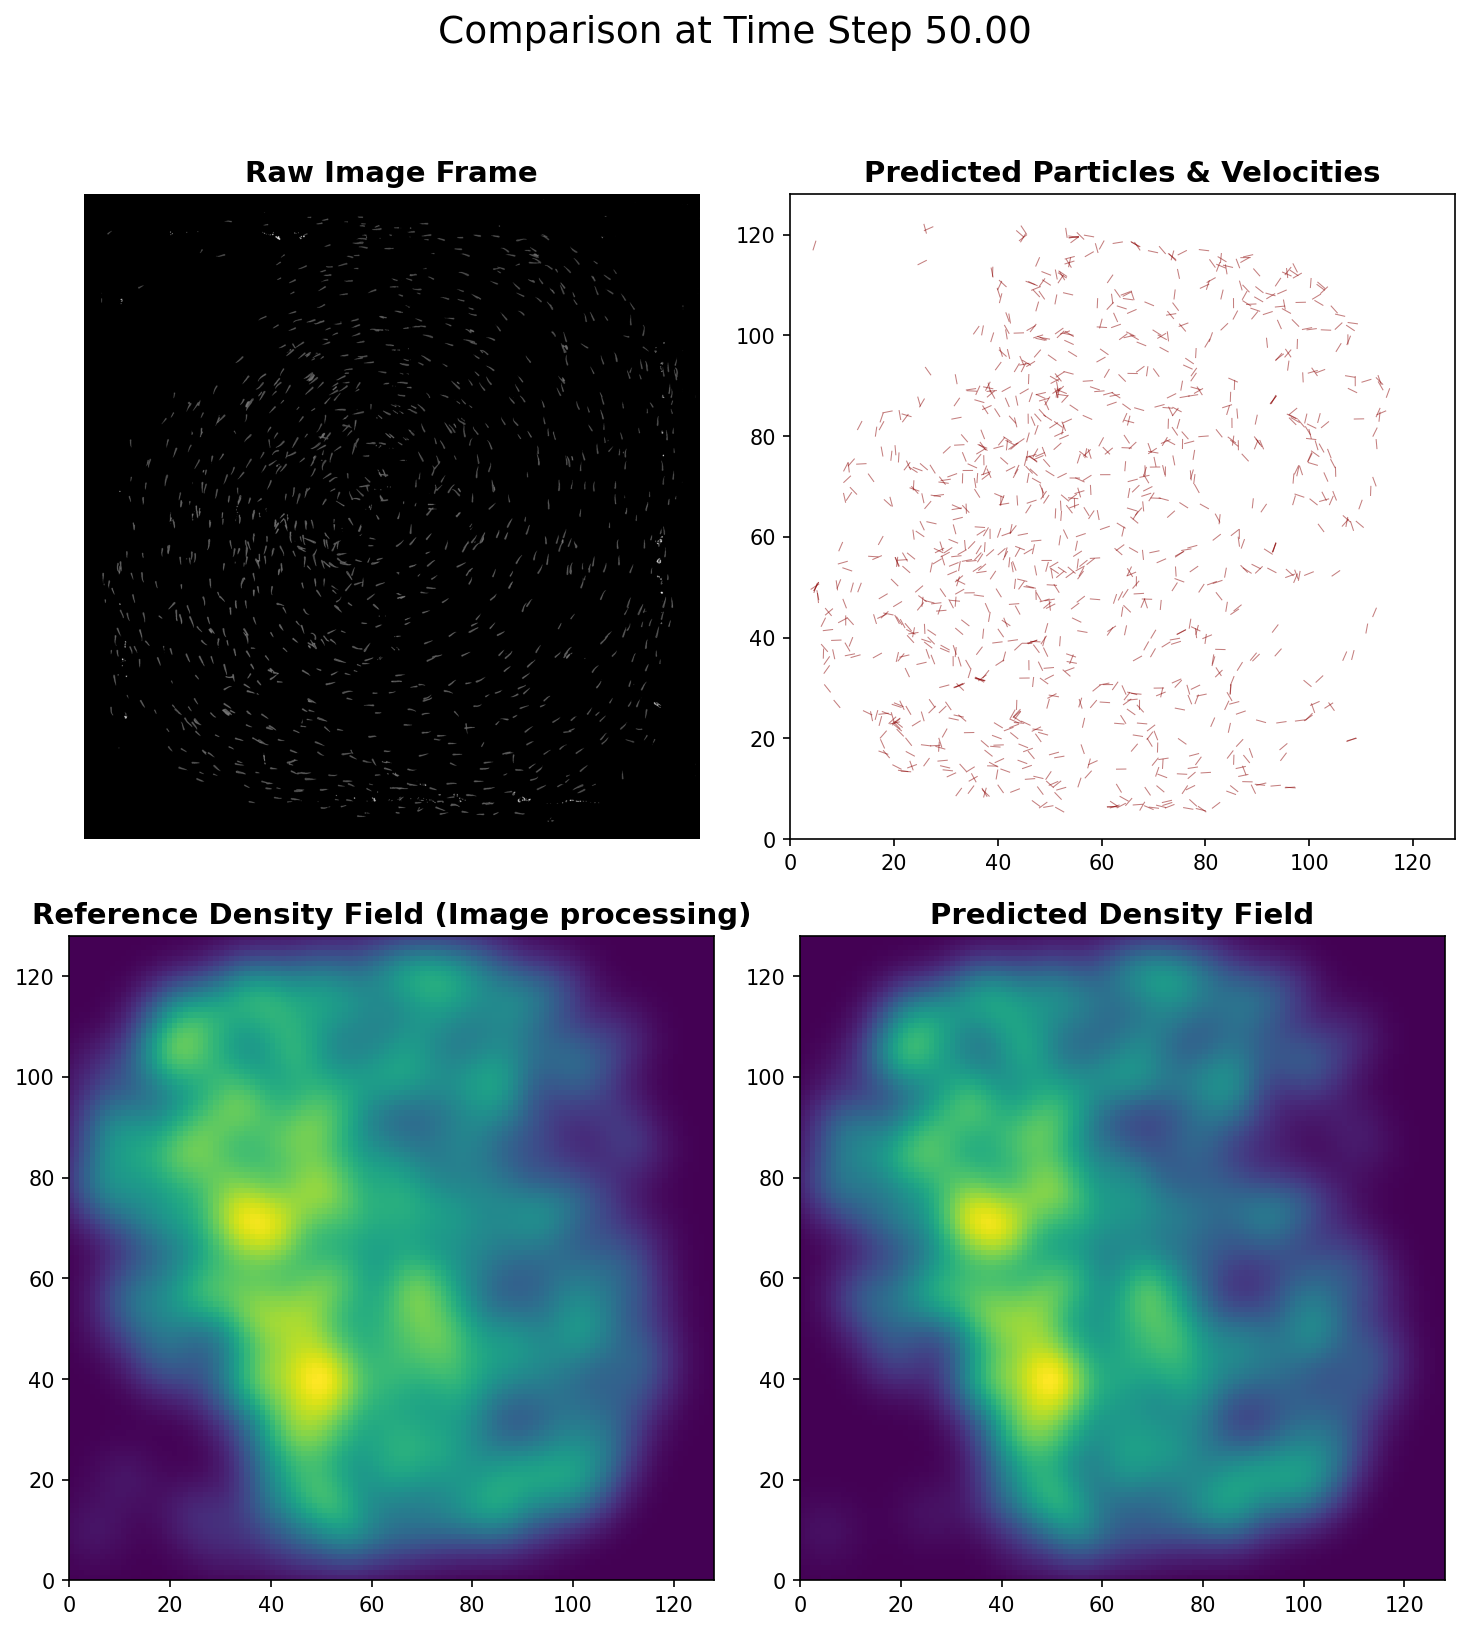
\includegraphics[width=0.9\linewidth]{figure/comparison_2x2_density.png}
    \caption{\textbf{Collective-motion data example at time step \(50\).}
    Top-left: raw image frame. Top-right: assimilated particle positions
    and velocities. Bottom-left: reference density reconstructed from
    image processing. Bottom-right: density of the corrected particle
    system. The assimilated forecast reproduces the dominant macroscopic
    organization observed in the experiment.}
    \label{fig:fish_t_50}
\end{figure}

Overall, the numerical experiments exhibit a consistent pattern.
Increasing \(\lambda\) improves agreement with the reference solution
across linear, nonlinear, chaotic, and real-data settings, while
excessively large feedback can introduce stiffness or transient
oscillations. This trade-off matches the analysis in Section~2: the
nudging must be strong enough to overcome model bias, but its strength
must remain compatible with the observation resolution and the numerical
discretization.






\section{Conclusion}

We have introduced Multiscale Nudge, a cross-scale data assimilation
framework that feeds macroscopic density observations back into
microscopic mean-field dynamics. The nudging term arises as the
Wasserstein gradient of a regularised observation-misfit functional and
admits a direct particle implementation that requires neither tangent
linear models nor ensemble bookkeeping. On the theoretical side, we
proved well-posedness and propagation of chaos for the assimilated
particle system, and showed that the $L^2$ error between the true and
assimilated densities decays exponentially to a bias floor controlled by
the model misspecification~$\Delta$. On the numerical side, experiments
spanning linear, bimodal, chaotic, kinetic, and real collective-motion
systems demonstrated that the method consistently improves forecast
accuracy from smoothed density observations alone.
